% =============================================================================
%  Rapport Promptly — Utilisation de l'intelligence artificielle
%  Compiler : latexmk -pdf main.tex   OU   pdflatex main.tex (x2)
% =============================================================================
\documentclass[11pt,a4paper]{report}

\usepackage[utf8]{inputenc}
\usepackage[T1]{fontenc}
\usepackage[french]{babel}
\usepackage{geometry}
\usepackage{graphicx}
\usepackage{hyperref}
\usepackage{booktabs}
\usepackage{longtable}
\usepackage{enumitem}
\usepackage{xcolor}
\usepackage{listings}
\usepackage{float}
\usepackage{caption}
\usepackage{fancyhdr}
\usepackage{titlesec}

\geometry{margin=2.5cm}
\hypersetup{
  colorlinks=true,
  linkcolor=black,
  urlcolor=blue,
  citecolor=black
}

\graphicspath{{figures/}{figures/chatgpt/}{figures/cursor/}{figures/app/}}

% Encadre pour les prompts
\usepackage{tcolorbox}
\tcbuselibrary{breakable,skins}
\newtcolorbox{promptbox}[1][]{
  colback=gray!8,
  colframe=gray!50,
  fonttitle=\bfseries,
  title={Prompt},
  breakable,
  #1
}
\newtcolorbox{resultbox}[1][]{
  colback=green!3,
  colframe=green!40!black,
  fonttitle=\bfseries,
  title={Resultat},
  breakable,
  #1
}
\newtcolorbox{problembox}[1][]{
  colback=red!3,
  colframe=red!40!black,
  fonttitle=\bfseries,
  title={Probleme},
  breakable,
  #1
}

\pagestyle{fancy}
\fancyhf{}
\fancyhead[L]{Promptly --- Rapport IA}
\fancyhead[R]{\thepage}
\renewcommand{\headrulewidth}{0.4pt}

\title{%
  Utilisation de l'intelligence artificielle\\
  dans le projet \textbf{Promptly}\\[1em]
  \large Rapport : outils d'IA (developpement) et IA integree au produit
}
\author{%
  Encadre par : \textbf{Khemiri Akram}\\[1.2em]
  \textbf{\'Equipe Alpha Code}\\[0.8em]
  Lamis Ben Hassine\\
  Khalil Fray\\
  Saif Denden\\
  Isra Bel Habib\\
  Hamza Taychi\\[1em]
  Annee universitaire 2025--2026
}
\date{\today}

\begin{document}

\maketitle

\begin{abstract}
Ce rapport documente l'utilisation de l'intelligence artificielle dans le projet
\textbf{Promptly}, une plateforme d'apprentissage en ligne (Spring Boot + Angular).
Deux axes sont distingues :
\begin{enumerate}
  \item l'\textbf{IA comme outil de developpement} (ChatGPT, puis editeur Cursor
        avec modeles Claude, Grok, etc.), avec prompts, resultats, corrections
        et captures d'ecran ;
  \item l'\textbf{IA integree a l'application} (Ollama, APIs externes, microservices ML),
        avec justification, fonctionnement et resultats observes.
\end{enumerate}
\end{abstract}

\tableofcontents
\newpage

\chapter{Introduction}
\label{ch:intro}

\section{Objectif du rapport}

Ce rapport documente l'utilisation de l'intelligence artificielle dans le projet
\textbf{Promptly}. Il presente :
\begin{itemize}
  \item les \textbf{outils d'IA} utilises pour concevoir et coder l'application ;
  \item les \textbf{fonctionnalites d'IA} integrees au produit livre.
\end{itemize}

\section{Deux faces de l'IA}

\begin{enumerate}
  \item \textbf{IA cote developpement.} ChatGPT a servi a preparer le premier
        grand prompt. L'editeur \textbf{Cursor} (mode Agent) a ensuite heberge
        le dialogue avec des \textbf{modeles} tels que \textbf{Claude} et
        \textbf{Grok}, qui ont genere, corrige et explique le code. Chaque etape
        importante est documentee : prompt, resultat, eventuel probleme, prompt
        de correction, nouveau resultat --- avec captures d'ecran.
  \item \textbf{IA cote application.} Le produit appelle des modeles et des APIs
        (Ollama, Hugging Face, Sightengine, TextGears, Gemini, services ML locaux)
        pour resume, chat, moderation, emotion, matching CV, etc.
\end{enumerate}

\section{Methode de documentation}

Pour chaque echange significatif avec une IA de developpement :
\begin{enumerate}
  \item capture du \textbf{prompt} ;
  \item capture du \textbf{resultat} ;
  \item si erreur ou ecart : capture du \textbf{probleme}, du \textbf{prompt de
        correction}, puis du \textbf{resultat corrige}.
\end{enumerate}

Les images sont placees dans \texttt{figures/chatgpt/}, \texttt{figures/cursor/}
et \texttt{figures/app/}.

\section{Organisation du document}

Le chapitre~\ref{ch:role} rappelle brievement le role de Promptly.
Le chapitre~\ref{ch:dev} detaille la chaine ChatGPT~$\rightarrow$~Cursor
(Claude / Grok).
Le chapitre~\ref{ch:app} presente l'IA integree au produit.
Le chapitre~\ref{ch:conclusion} conclut.

% --- Contenu a completer apres validation ---

\chapter{Role du projet Promptly}
\label{ch:role}

\section{Contexte}

\textbf{Promptly} est une plateforme web d'apprentissage dediee a la programmation
(Java, Spring Boot, Angular, algorithmique). Elle s'adresse aux etudiants, aux
enseignants et a un administrateur.

\section{Fonctionnalites principales}

\begin{itemize}
  \item \textbf{Cours et chapitres} : contenus, PDF, resume IA, flashcards ;
  \item \textbf{Quiz} : QCM, scores, detection GUESS/KNOW (ML) ;
  \item \textbf{Forum} : discussions, auto-correction (TextGears), censure (Sightengine) ;
  \item \textbf{Reclamations} : depot etudiant, labels ML + emotion (admin) ;
  \item \textbf{Recrutement} : offres (admin), candidature + CV, matching competences (Gemini) ;
  \item \textbf{Assistant IA} : chatbot general (Ollama).
\end{itemize}

\section{Pile technique}

\begin{table}[H]
\centering
\begin{tabular}{@{}ll@{}}
\toprule
Couche & Technologie \\
\midrule
Frontend & Angular \\
Backend & Spring Boot 3 \\
Base de donnees & MySQL \\
LLM local & Ollama \\
ML locaux & Python (FastAPI) --- ports 8090 / 8091 \\
\bottomrule
\end{tabular}
\caption{Pile technique de Promptly}
\end{table}

\section{Roles utilisateurs}

\begin{itemize}
  \item \textbf{ETUDIANT} : cours, quiz, forum, reclamations, candidatures, assistant ;
  \item \textbf{ENSEIGNANT} : gestion des cours / quiz (+ meme acces apprenant) ;
  \item \textbf{ADMIN} : utilisateurs, traitement reclamations, offres de recrutement, vues ML.
\end{itemize}

\chapter{IA utilisee pour developper le projet}
\label{ch:dev}

\section{Outils et modeles}

Il faut distinguer l'\textbf{environnement} (ou l'on ecrit les prompts) et le
\textbf{modele d'IA} (qui produit les reponses).

\begin{table}[H]
\centering
\begin{tabular}{@{}p{3.5cm}p{9.5cm}@{}}
\toprule
Element & Role \\
\midrule
\textbf{ChatGPT} (web) &
Premier echange : expression du besoin ; generation du prompt structure
a coller ensuite dans Cursor. \\
\textbf{Cursor} &
Editeur / IDE (mode Agent) : interface de chat, fichiers du projet, terminal.
Ce n'est pas le modele lui-meme. \\
\textbf{Claude} (Anthropic) &
Modele utilise dans Cursor pour generer et corriger le code
(ex.\ Claude~5.5 / Sonnet). \\
\textbf{Grok} (xAI) &
Autre modele propose dans Cursor, egalement utilise selon les besoins. \\
\bottomrule
\end{tabular}
\caption{Outils (environnement) et modeles d'IA de developpement}
\end{table}

En resume : \textbf{Cursor = editeur} ; \textbf{Claude / Grok = IA} qui repondent
aux prompts a l'interieur de Cursor. ChatGPT a ete utilise en amont pour preparer
le premier prompt. Les sessions ci-dessous sont reconstituees a partir de
l'\textbf{historique de chat} Cursor (prompts reels + resultats observes).

\section{Chaine initiale : ChatGPT puis Cursor}
\label{sec:chatgpt-cursor}

\subsection{Prompt de l'auteur a ChatGPT}

\begin{promptbox}[title={Prompt utilisateur $\rightarrow$ ChatGPT}]
i will make acadamique project so the project about elearning named promptly
for giving courses about coding like springboot java angular \ldots{} and
algorithme the gestion of the project is reclamation, cours and chapter,
evaluation like small test quiz, forome like samll comunite all the student
will make postes and told to each other so this project about how to use the
ia to make the project like i use currsor or chatgpt the prffesor told as to
give he screen shot of the promte and the result after the prompt and
correction of the promte if we need it and also how we use the ia in the
project like how we use olama if we work with it and how we use api extern in
the project exetera bacouse we will make rapport about this in the end so
give me promte give it to the currsor to make this and dont forget the
content of the rapport becouse if we need screenshot lets make it to put in
in the rapport like i tolde u the part how we use ia in the porcet and how we
use ia to make the project also told him to begin with the template then we
need to make gestion by gestion don't make the full project in one prmote the
project with springboot and angular lets begin with the template then make
the other gestion step by step each step need confiramtion
\end{promptbox}

\begin{figure}[H]
  \centering
  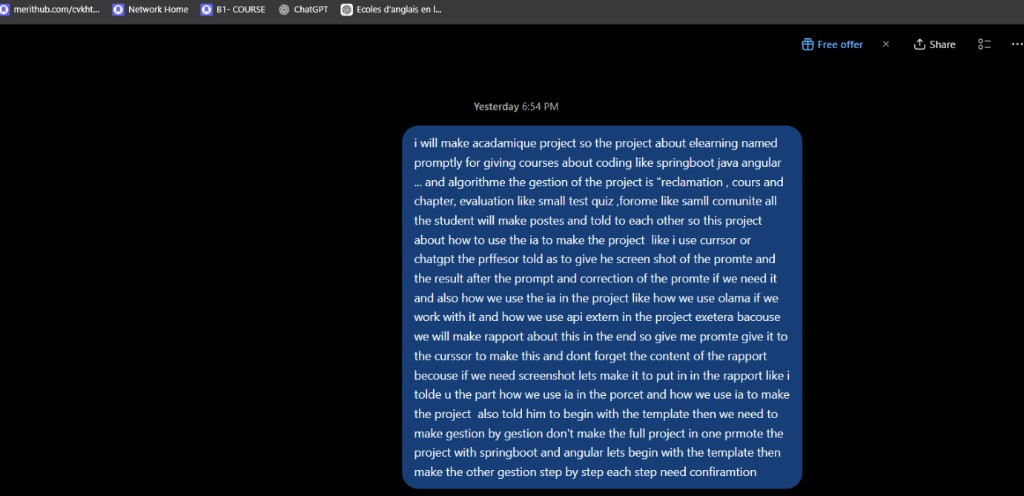
\includegraphics[width=0.92\textwidth]{chatgpt/01-prompt-utilisateur.png}
  \caption{Capture --- premier prompt envoye a ChatGPT}
  \label{fig:chatgpt-prompt}
\end{figure}

\subsection{Resultat ChatGPT : prompt pour Cursor}

\begin{resultbox}[title={Reponse ChatGPT --- resume du prompt pour Cursor}]
\textbf{Stack.} Backend : Java~17, Spring Boot, Web, JPA, Security, Validation,
Maven, MySQL. Frontend : Angular, TypeScript, Router, services, Reactive Forms,
UI responsive.

\textbf{Architecture.} Monolithe : un backend Spring Boot, un frontend Angular,
une base MySQL. Packages classiques ; pas de microservices.

\textbf{Contraintes.} Interdit : Eureka, API Gateway, Docker/Kubernetes.
Execution locale ; Spring Boot connecte directement a MySQL.

\textbf{IA (plus tard).} Ollama et APIs externes seulement apres validation.

\textbf{Workflow etape~1 (template).} Initialiser Spring Boot + Angular,
MySQL, page d'accueil, health-check ; attendre confirmation avant chaque
module suivant.
\end{resultbox}

\begin{figure}[H]
  \centering
  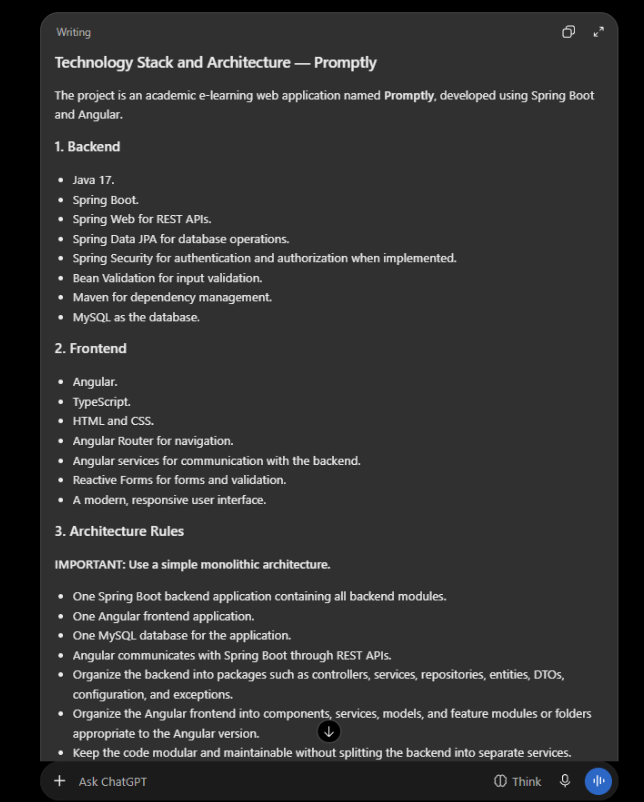
\includegraphics[width=0.92\textwidth]{chatgpt/02a-reponse-chatgpt-stack.png}
  \caption{Capture --- prompt Cursor genere par ChatGPT (stack et architecture)}
  \label{fig:chatgpt-result-stack}
\end{figure}

\begin{figure}[H]
  \centering
  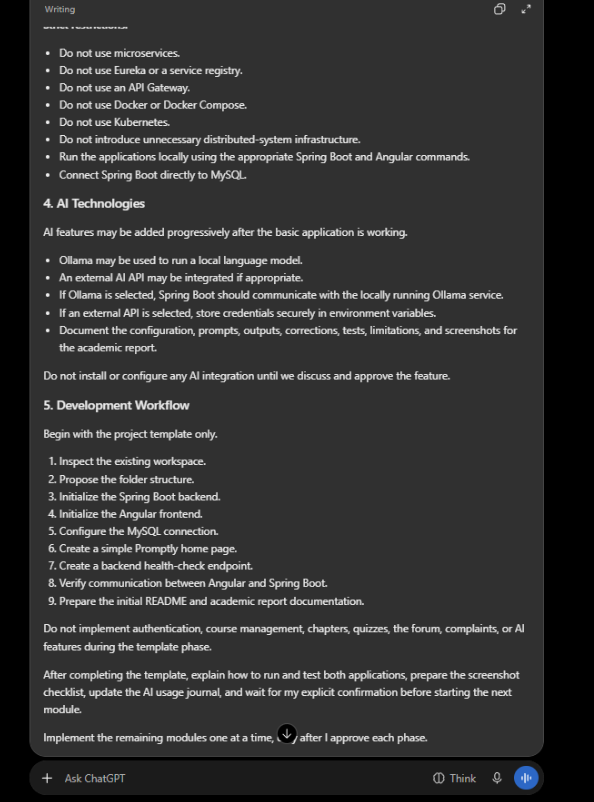
\includegraphics[width=0.92\textwidth]{chatgpt/02b-reponse-chatgpt-workflow.png}
  \caption{Capture --- suite du prompt Cursor (contraintes, IA, workflow template)}
  \label{fig:chatgpt-result-workflow}
\end{figure}

\section{Sessions Cursor par gestion}
\label{sec:sessions-cursor}

Chaque sous-section = une \textbf{gestion} (ou un lot de prompts lies).
Format : \textbf{Prompt} $\rightarrow$ \textbf{Resultat}
(et corrections si un probleme a ete corrige dans le chat).
Modele dans Cursor : \textbf{Claude~5.5} / \textbf{Grok} (selon la session).

%----------------------------------------------------------------------
\subsection{S0 --- Fondation (template Spring Boot + Angular)}
\label{sec:s0}

\textbf{Modele :} Claude / Grok (Cursor Agent)

\begin{promptbox}[title={Prompt (issu de ChatGPT, colle dans Cursor)}]
Academic E-Learning Project --- Promptly. Develop progressively,
management by management, confirm each step. Phase~0 / template only:
inspect workspace, propose folder structure, initialize Spring Boot backend,
Angular frontend, configure MySQL, simple Promptly home page, health-check
endpoint, verify Angular~$\leftrightarrow$~Spring Boot. Do not implement
auth, courses, quizzes or AI yet.
\end{promptbox}

\begin{resultbox}[title={Resultat}]
Workspace initialise : backend Spring Boot (Maven, MySQL, \texttt{/api/health}),
frontend Angular, README. Communication Angular~$\leftrightarrow$~API verifiee.
Attente de confirmation avant le module suivant.
\end{resultbox}

\begin{figure}[H]
  \centering
  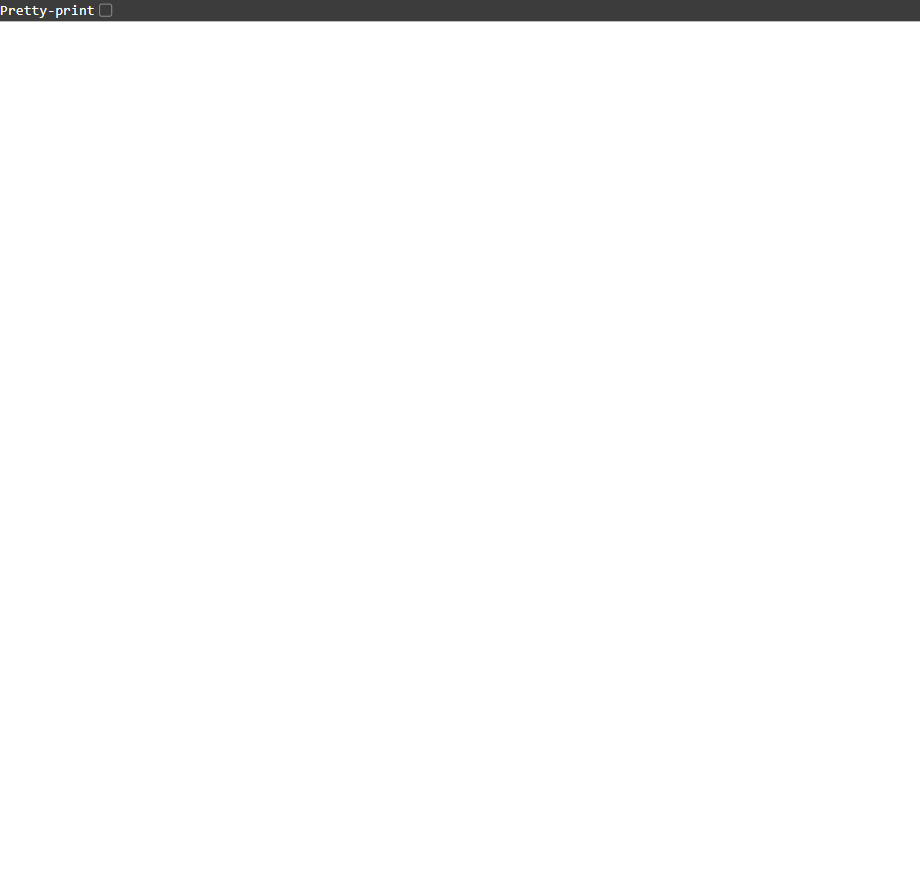
\includegraphics[width=0.92\textwidth]{app/S0-health-api.png}
  \caption{Capture Promptly --- health-check API (\texttt{/api/health})}
  \label{fig:s0-health}
\end{figure}

%----------------------------------------------------------------------
\subsection{S1 --- Authentification et utilisateurs}
\label{sec:s1}

\begin{promptbox}
Implement Module~1 --- Authentication and User Management:
registration, login, JWT, roles (ETUDIANT / ENSEIGNANT / ADMIN),
admin user list, access restrictions.
\end{promptbox}

\begin{resultbox}[title={Resultat}]
Auth complete : inscription, login JWT, roles, page admin utilisateurs.
Tests backend \texttt{BUILD SUCCESS} ; routes protegees (\texttt{401}/\texttt{403}
verifies). Compte admin initialise via variables d'environnement.
\end{resultbox}

\begin{figure}[H]
  \centering
  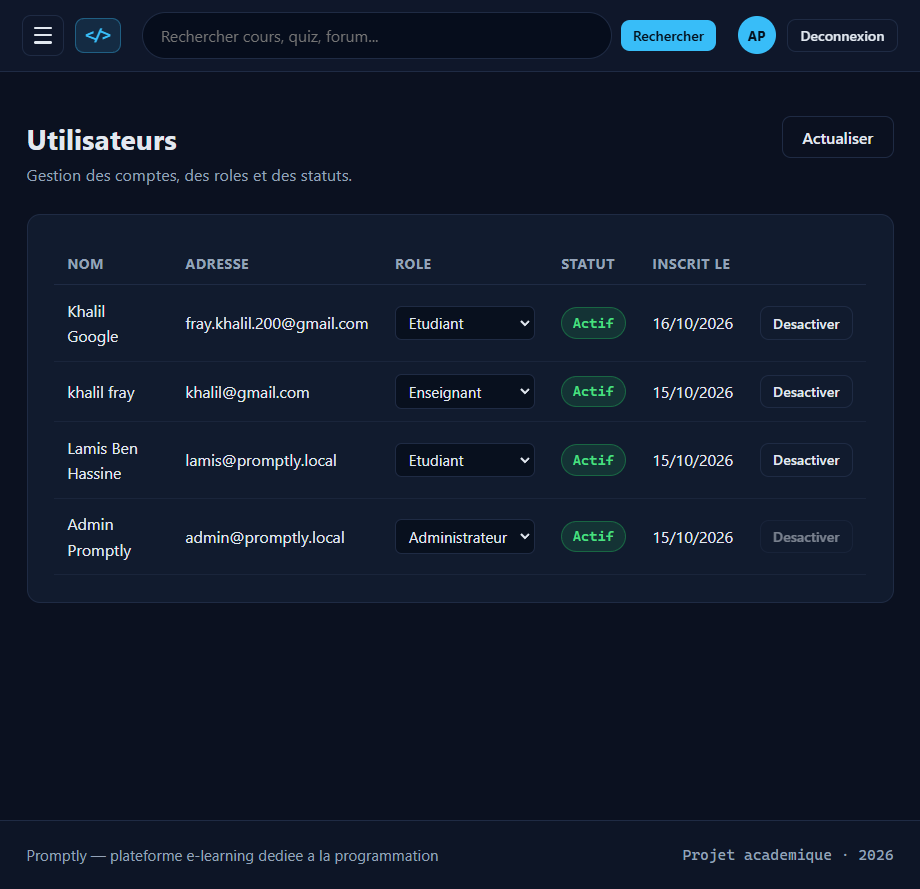
\includegraphics[width=0.92\textwidth]{app/S1-admin-utilisateurs.png}
  \caption{Capture Promptly --- administration des utilisateurs}
  \label{fig:s1-users}
\end{figure}

\begin{promptbox}[title={Prompt suivant --- Google Sign-In}]
lets make in the user part login with gmail make the code and tell me what
i have to add like i have to take token \ldots
\end{promptbox}

\begin{resultbox}[title={Resultat}]
Bouton Google sur Connexion / Inscription. Frontend envoie l'ID token a
\texttt{POST /api/auth/google} ; backend verifie avec le Client~ID puis
emet le JWT Promptly. Configuration :
\texttt{googleClientId} (frontend) + \texttt{PROMPTLY\_GOOGLE\_CLIENT\_ID}.
\end{resultbox}

\begin{figure}[H]
  \centering
  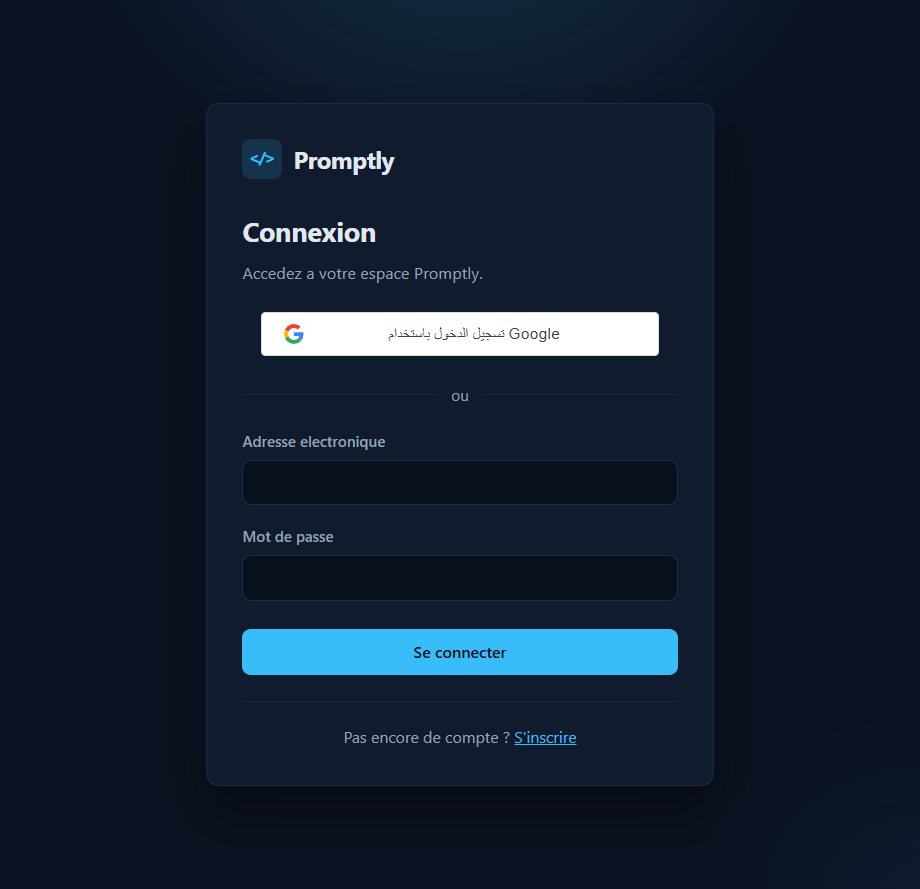
\includegraphics[width=0.75\textwidth]{app/S1-google-login.png}
  \caption{Capture Promptly --- Connexion avec bouton Google}
  \label{fig:s1-google}
\end{figure}

\begin{promptbox}[title={Prompt --- page d'accueil}]
the first page make it like login or gigin up olny without the nav and side bar
\end{promptbox}

\begin{resultbox}[title={Resultat}]
\texttt{/} redirige vers Connexion (ou Cours si deja connecte).
Pages Connexion / Inscription sans navbar ni sidebar.
Bouton Google visible sur la page de connexion.
\end{resultbox}

\begin{figure}[H]
  \centering
  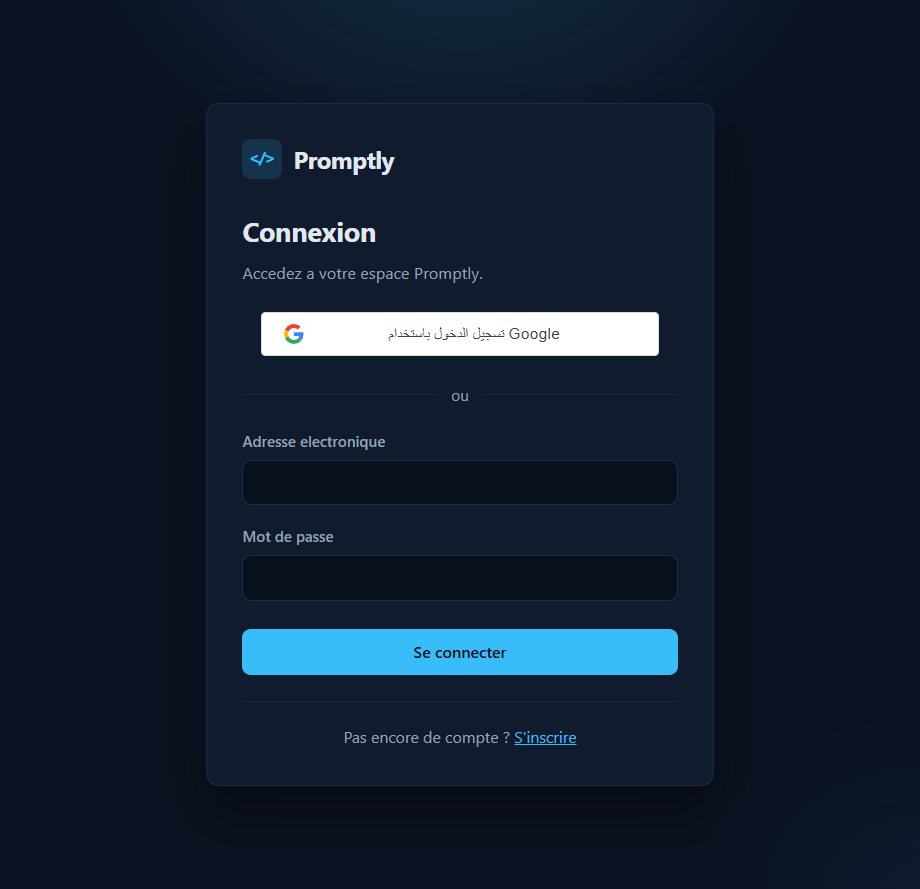
\includegraphics[width=0.75\textwidth]{app/S1-connexion.png}
  \caption{Capture Promptly --- page Connexion (sans nav/sidebar) + Google}
  \label{fig:s1-login}
\end{figure}

%----------------------------------------------------------------------
\subsection{S2 --- Cours et chapitres}
\label{sec:s2}

\begin{promptbox}
implement module 2
\end{promptbox}

\begin{resultbox}[title={Resultat}]
CRUD cours : categories (Java, Spring Boot, Angular, \ldots), publication,
roles (etudiant = publies ; enseignant = ses cours ; admin = tous).
Routes \texttt{/cours}, formulaires, catalogue filtre.
\end{resultbox}

\begin{figure}[H]
  \centering
  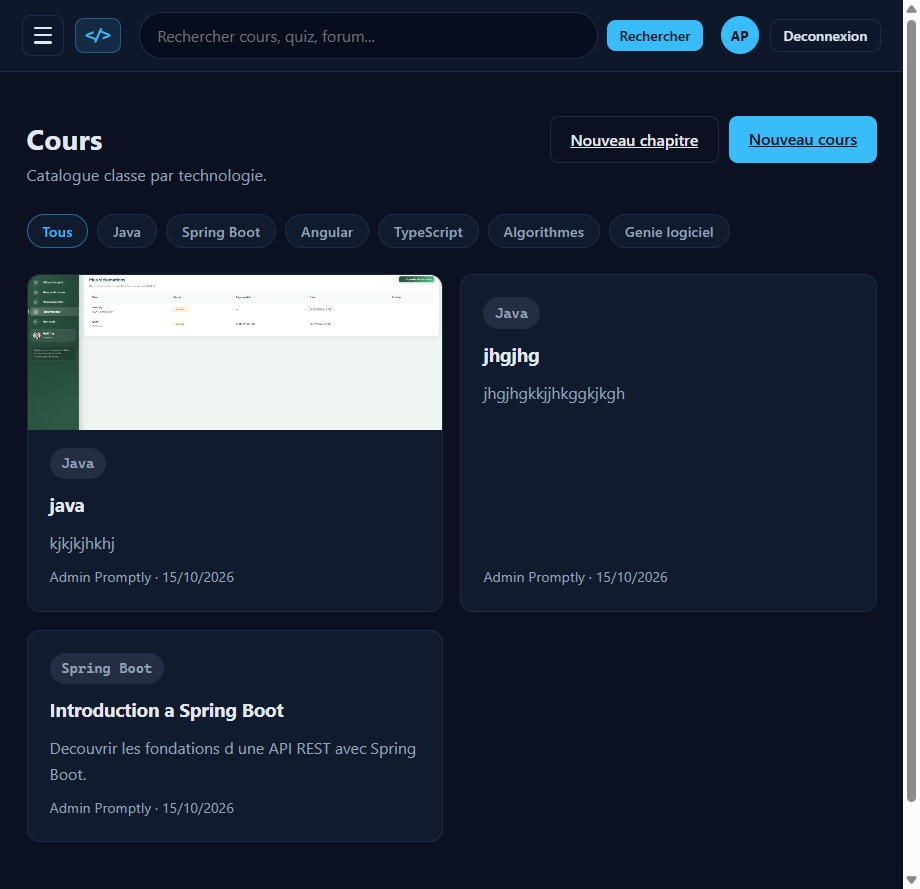
\includegraphics[width=0.92\textwidth]{app/S2-cours-catalogue.png}
  \caption{Capture Promptly --- catalogue des cours}
  \label{fig:s2-cours}
\end{figure}

\begin{promptbox}
add img to the cours and upload pdf to the cours and chapter to the cours
\end{promptbox}

\begin{resultbox}[title={Resultat}]
Upload image de couverture + PDF cours ; chapitres lies au cours avec PDF ;
fichiers servis via \texttt{/api/files/**} (dossier \texttt{uploads/}).
\end{resultbox}

\begin{figure}[H]
  \centering
  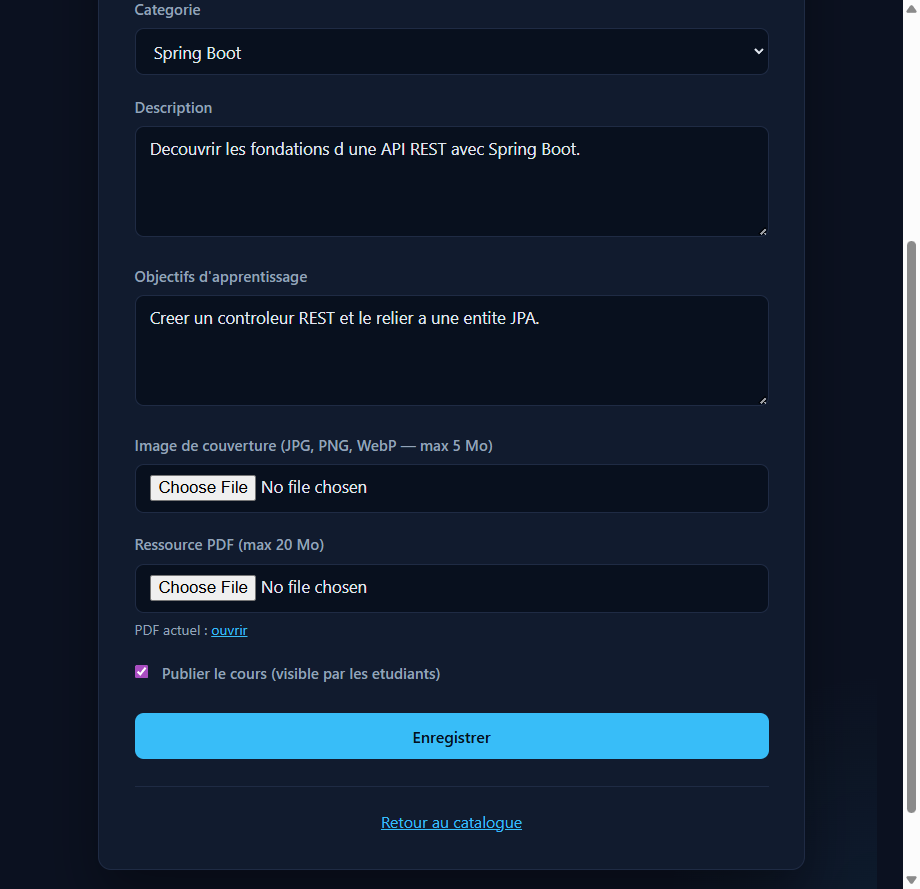
\includegraphics[width=0.92\textwidth]{app/S2-cours-form-media.png}
  \caption{Capture Promptly --- formulaire cours (image de couverture + PDF)}
  \label{fig:s2-media}
\end{figure}

\begin{promptbox}
make it when i add chapter i choose the cours of the chapter
\end{promptbox}

\begin{resultbox}[title={Resultat}]
Formulaire << Nouveau chapitre >> avec liste deroulante de cours
(presaisie si on vient d'une fiche cours).
\end{resultbox}

\begin{figure}[H]
  \centering
  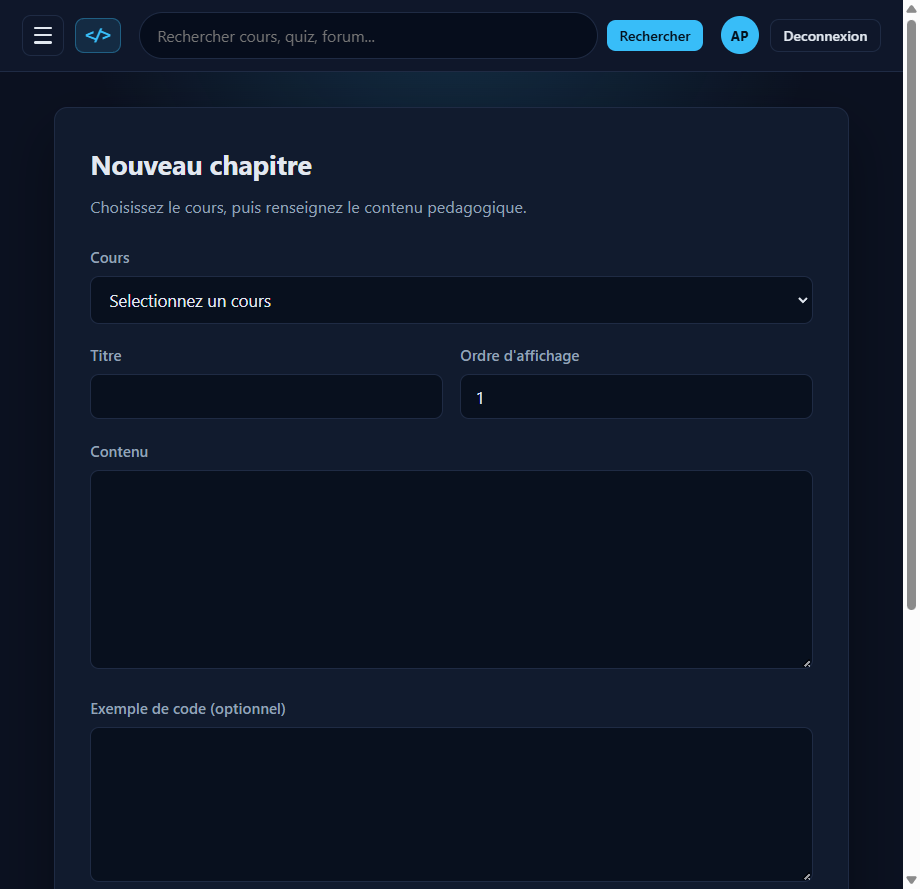
\includegraphics[width=0.92\textwidth]{app/S2-chapitre-form.png}
  \caption{Capture Promptly --- Nouveau chapitre (choix du cours)}
  \label{fig:s2-chapitre}
\end{figure}

%----------------------------------------------------------------------
\subsection{S3 --- Evaluations / Quiz}
\label{sec:s3}

\begin{promptbox}
MAKE THE NEXT GESTION
\end{promptbox}

\begin{resultbox}[title={Resultat}]
Module Quiz : QCM lies a un cours (chapitre optionnel), passage etudiant,
score ; enseignants voient les tentatives. Nav \texttt{/quiz}.
\end{resultbox}

\begin{figure}[H]
  \centering
  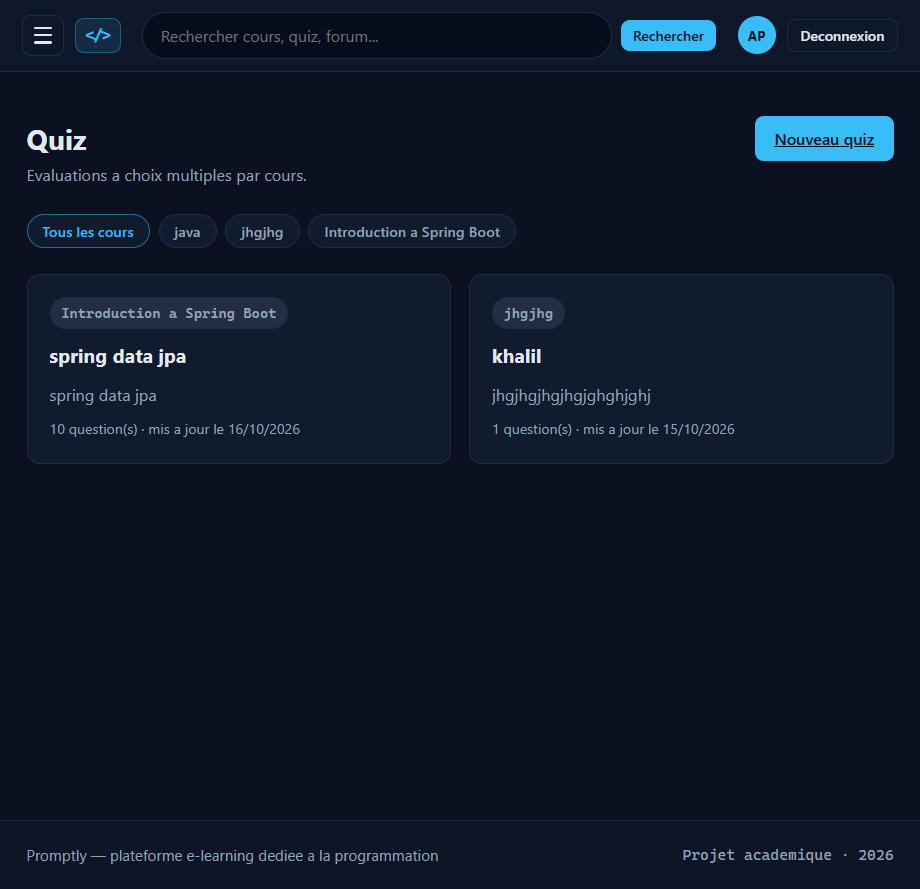
\includegraphics[width=0.92\textwidth]{app/S3-quiz-liste.png}
  \caption{Capture Promptly --- liste des quiz}
  \label{fig:s3-quiz-list}
\end{figure}

\begin{promptbox}
now i need to make in the evaluation generation quiez with ollma when i add
the titre and description and when i slect the cours of the quiz take all
this then tell the ollma to make quiz with 10 quetions
\end{promptbox}

\begin{resultbox}[title={Resultat}]
Bouton << Generer 10 questions avec IA >> : Ollama utilise titre, description
et contenu du cours/chapitre/PDF pour proposer 10 QCM a revoir avant creation.
\end{resultbox}

\begin{figure}[H]
  \centering
  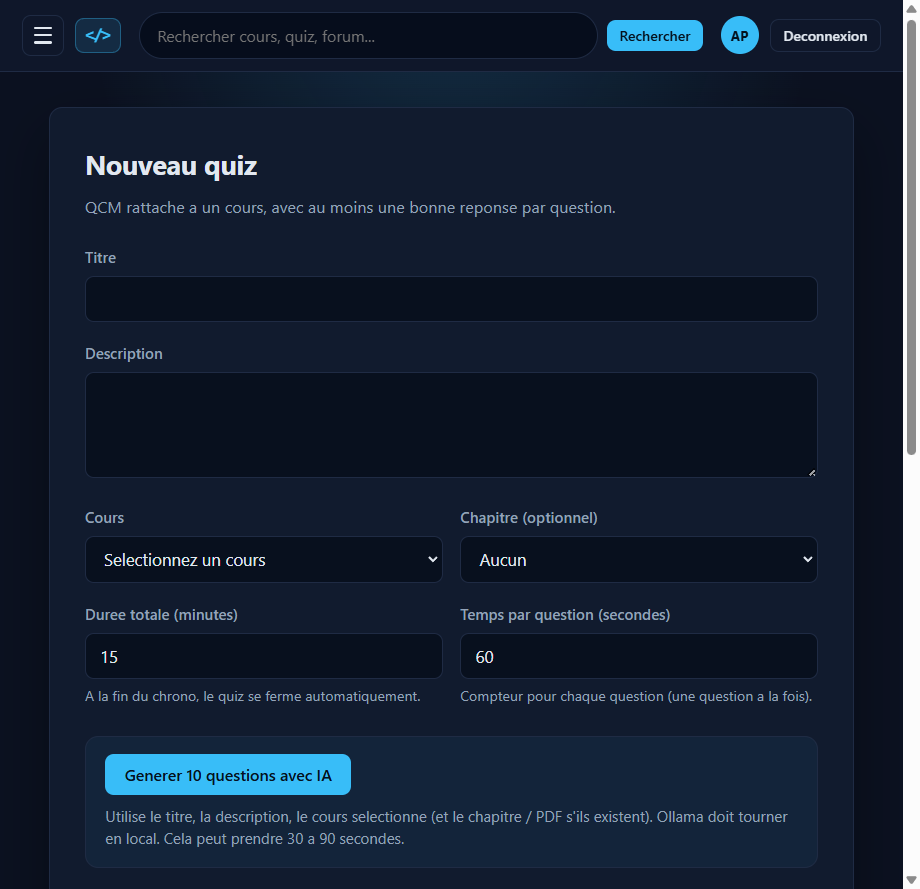
\includegraphics[width=0.92\textwidth]{app/S3-quiz-form-ia.png}
  \caption{Capture Promptly --- Nouveau quiz (timers + Generer 10 questions avec IA)}
  \label{fig:s3-quiz-form}
\end{figure}

\begin{figure}[H]
  \centering
  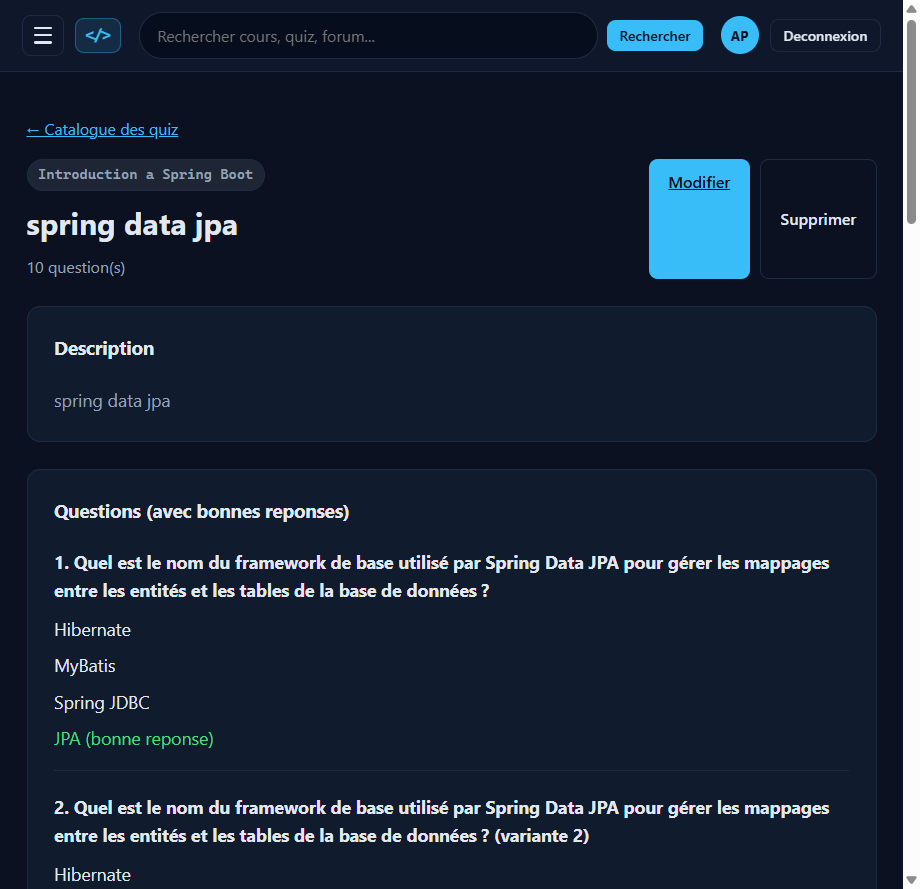
\includegraphics[width=0.92\textwidth]{app/S3-quiz-detail.png}
  \caption{Capture Promptly --- detail d'un quiz genere (questions + bonnes reponses)}
  \label{fig:s3-quiz-detail}
\end{figure}

\begin{promptbox}
make the student see the score nad the good reponse and the bad one and make
the techer can see all the student make the quiz with the result and maken him
can edit the result
\end{promptbox}

\begin{resultbox}[title={Resultat}]
Etudiant : score + correction (bonnes/mauvaises reponses). Enseignant :
liste des tentatives, detail, modification de note.
\end{resultbox}

\begin{figure}[H]
  \centering
  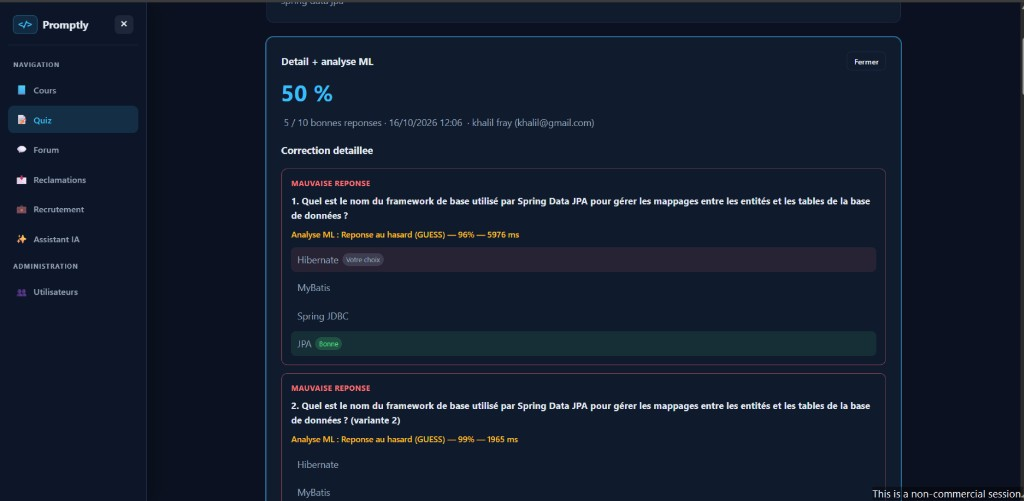
\includegraphics[width=0.92\textwidth]{app/S3-quiz-scores.png}
  \caption{Capture Promptly --- score et correction detaillee d'une tentative}
  \label{fig:s3-scores}
\end{figure}

\begin{promptbox}
make the quiz like this when i make the quiz i can add time when the time is
over the quiz will close and the quetion will come one by one not all the
quetion in the same page and make counter olso to each quetion then make
programe with machine learing then connect it to the prject the programe
predect the student when he check the answer he check it randomly or he know
the answer make onlly the techer see the guess or know the answer
\end{promptbox}

\begin{resultbox}[title={Resultat}]
Minuteur global + par question ; une question a la fois ; auto-soumission.
Service Python \texttt{ml-integrity} (port 8090, RandomForest) predit
\texttt{GUESS}/\texttt{KNOW} --- visible uniquement par l'enseignant.
\end{resultbox}

\begin{figure}[H]
  \centering
  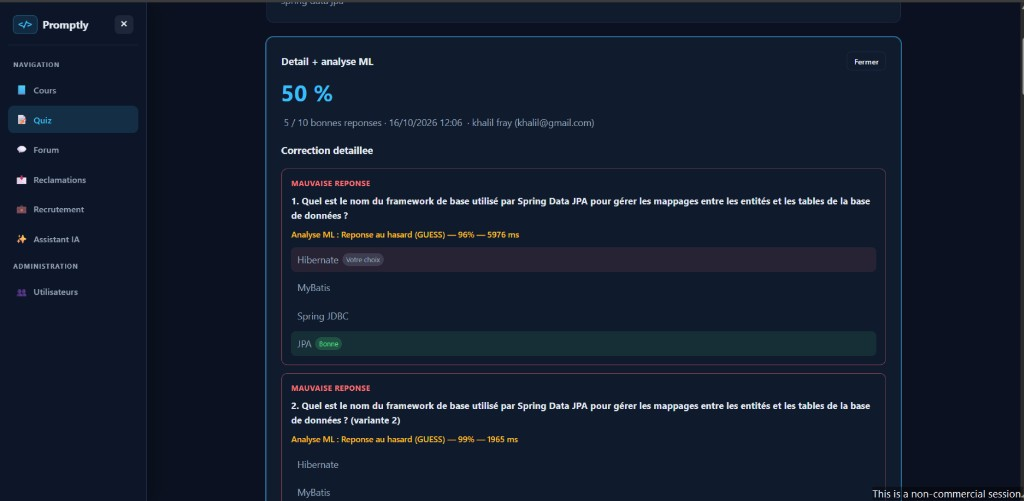
\includegraphics[width=0.92\textwidth]{app/S3-quiz-ml-guess-know.png}
  \caption{Capture Promptly --- Detail + analyse ML (labels GUESS / KNOW
  visibles uniquement pour l'enseignant)}
  \label{fig:s3-quiz-ml}
\end{figure}

\begin{problembox}[title={Probleme puis correction}]
\textbf{Prompt probleme :} when i click detail +ml no thing is happen \\
\textbf{Correction :} le panneau se mettait a jour hors ecran ; scroll +
section ML plus visible. \\
\textbf{Autre :} make modification when i make wrong reponse don't tell me he
know the reponse $\rightarrow$ reponse fausse forcee en \texttt{GUESS}.
\end{problembox}

%----------------------------------------------------------------------
\subsection{S4 --- Forum}
\label{sec:s4}

\begin{promptbox}
next gestion
\end{promptbox}

\begin{resultbox}[title={Resultat}]
Forum : sujets par categorie, commentaires, moderation / verrouillage
enseignants et admins. Nav \texttt{/forum}.
\end{resultbox}

\begin{figure}[H]
  \centering
  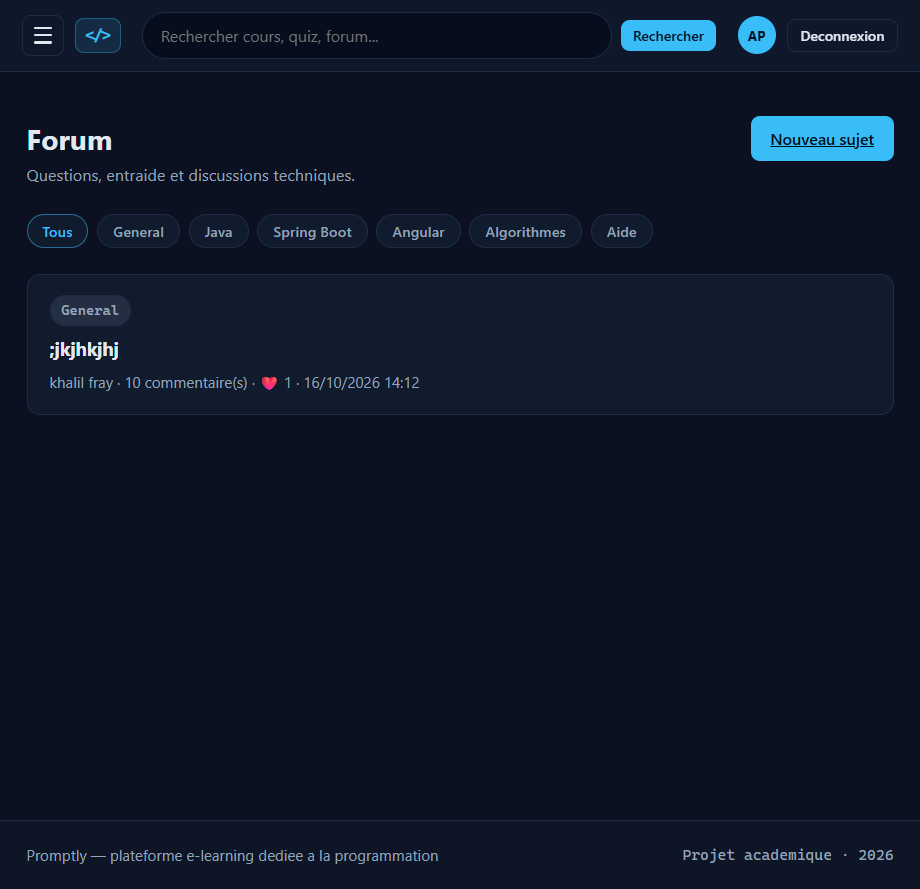
\includegraphics[width=0.92\textwidth]{app/S4-forum.png}
  \caption{Capture Promptly --- forum (sujets, categories, reactions)}
  \label{fig:s4-forum}
\end{figure}

\begin{promptbox}
add react to the forme like fb and img like fb post not just text
\end{promptbox}

\begin{resultbox}[title={Resultat}]
Posts avec image ; reactions type Facebook (like, coeur, rire, \ldots)
avec compteurs.
\end{resultbox}

\begin{figure}[H]
  \centering
  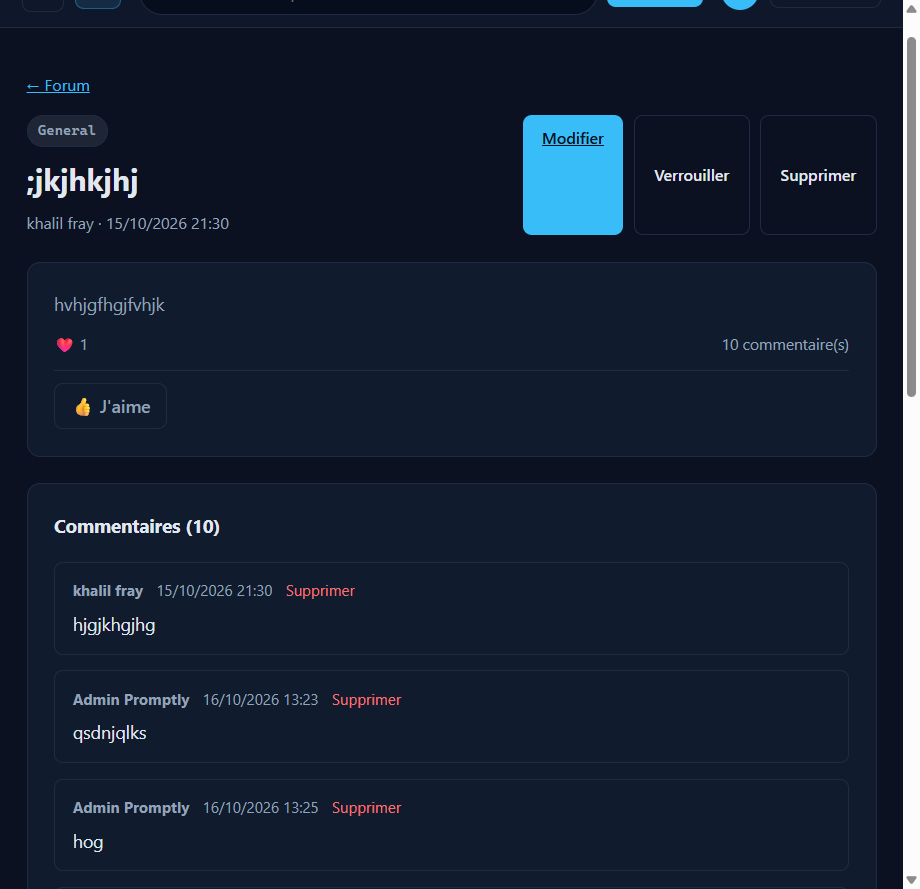
\includegraphics[width=0.92\textwidth]{app/S4-forum-detail-reactions.png}
  \caption{Capture Promptly --- detail sujet forum (reactions J'aime, commentaires)}
  \label{fig:s4-reactions}
\end{figure}

\begin{promptbox}
ok in the formome add api for badword bllocker \ldots make it with free one
\end{promptbox}

\begin{resultbox}[title={Resultat (apres choix API a token)}]
Moderation via \textbf{Sightengine} (api\_user + api\_secret). Insultes
remplacees par \texttt{***} (au lieu d'un rejet).
\end{resultbox}

\begin{figure}[H]
  \centering
  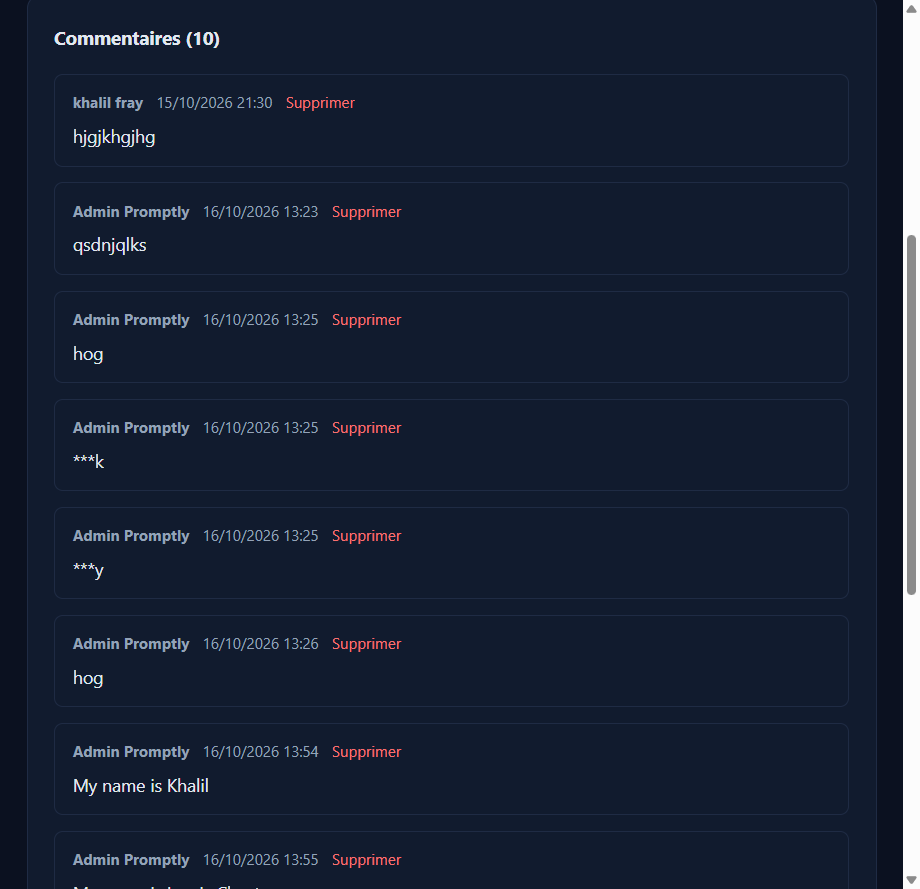
\includegraphics[width=0.92\textwidth]{app/S4-forum-moderation-stars.png}
  \caption{Capture Promptly --- commentaires avec censure \texttt{***} (Sightengine)}
  \label{fig:s4-stars}
\end{figure}

\begin{promptbox}
i need just when i type same thing wrong will auto correct when i post i need
api with token make this and free
\end{promptbox}

\begin{problembox}[title={Probleme --- APIs}]
GrammarBot annonce sa fermeture ; LanguageTool Premium refuse.
\textbf{Correction prompt :} don't do that the professor told us make api do
the auto correct $\rightarrow$ integration \textbf{TextGears} (cle API gratuite).
\end{problembox}

\begin{resultbox}[title={Resultat}]
A la publication d'un post/commentaire : correction orthographe TextGears
(FR/EN configurable), puis censure Sightengine \texttt{***}.
Champ de reponse : << Votre reponse (insultes $\rightarrow$ ***) >>.
\end{resultbox}

\begin{figure}[H]
  \centering
  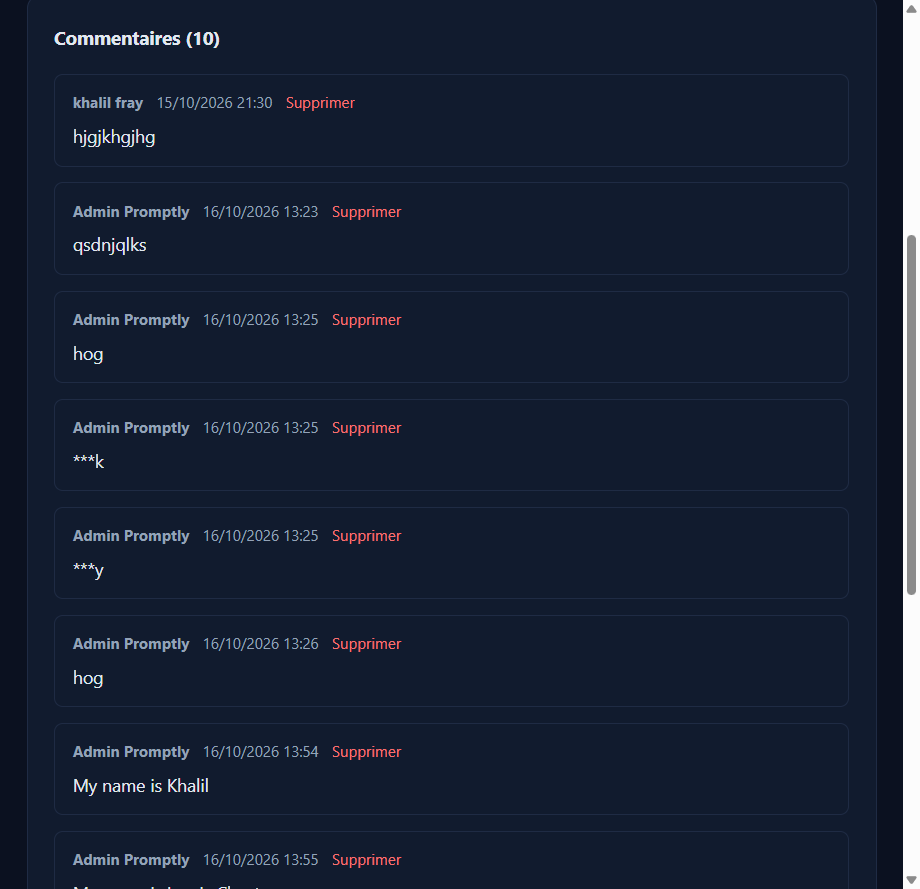
\includegraphics[width=0.92\textwidth]{app/S4-forum-moderation-stars.png}
  \caption{Capture Promptly --- moderation forum (TextGears + Sightengine \texttt{***})}
  \label{fig:s4-textgears}
\end{figure}

%----------------------------------------------------------------------
\subsection{S5 --- Reclamations}
\label{sec:s5}

\begin{promptbox}
good make the next one
\end{promptbox}

\begin{resultbox}[title={Resultat}]
Module reclamations : depot etudiant, suivi de statut ; admin repond et
change statut (\texttt{OUVERTE} $\rightarrow$ \texttt{EN\_COURS} $\rightarrow$
\texttt{RESOLUE}/\texttt{REJETEE}).
\end{resultbox}

\begin{figure}[H]
  \centering
  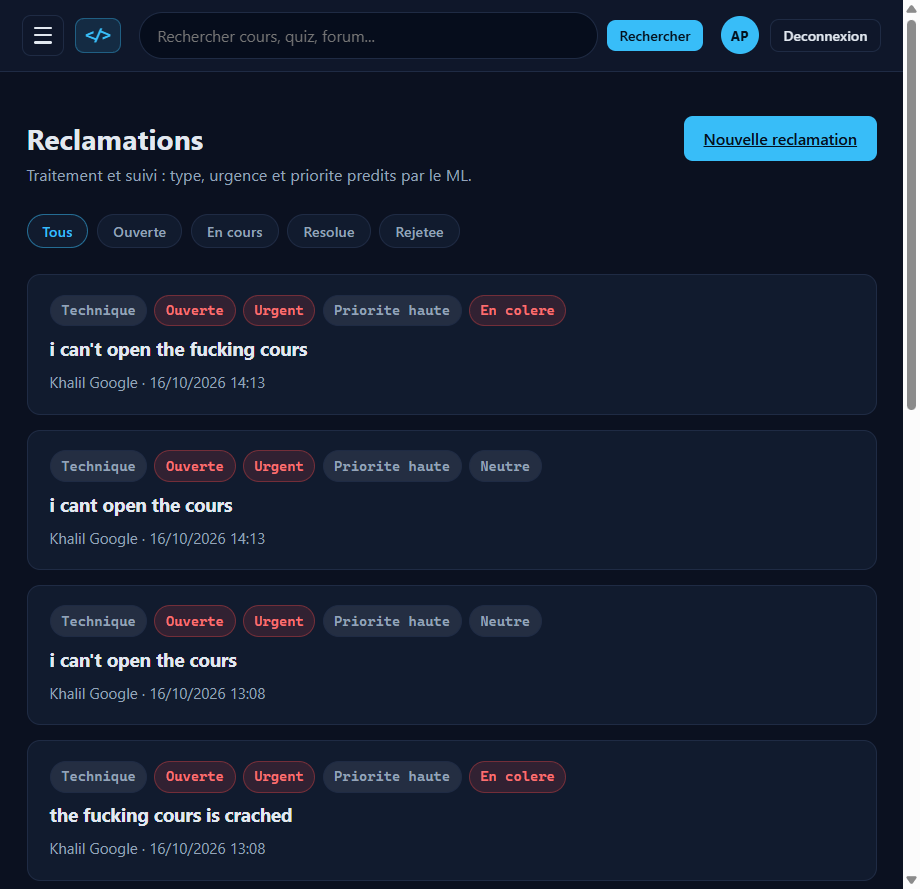
\includegraphics[width=0.92\textwidth]{app/S5-reclamations-liste.png}
  \caption{Capture Promptly --- liste des reclamations (filtres de statut)}
  \label{fig:s5-liste}
\end{figure}

\begin{promptbox}
in the reclamation make other machine learing when same one make reclamtion
the ml can classified urgence not urgence wand give each reclamtion preority
and and the type the reclamtion technique disponibility exetera the admine
can see this the user how make reclamtion he just make the reclamation
\end{promptbox}

\begin{resultbox}[title={Resultat}]
Service \texttt{ml-complaints} (port 8091) : type, urgence, priorite.
Visible admin seulement ; l'etudiant ne remplit que objet + description.
\end{resultbox}

\begin{figure}[H]
  \centering
  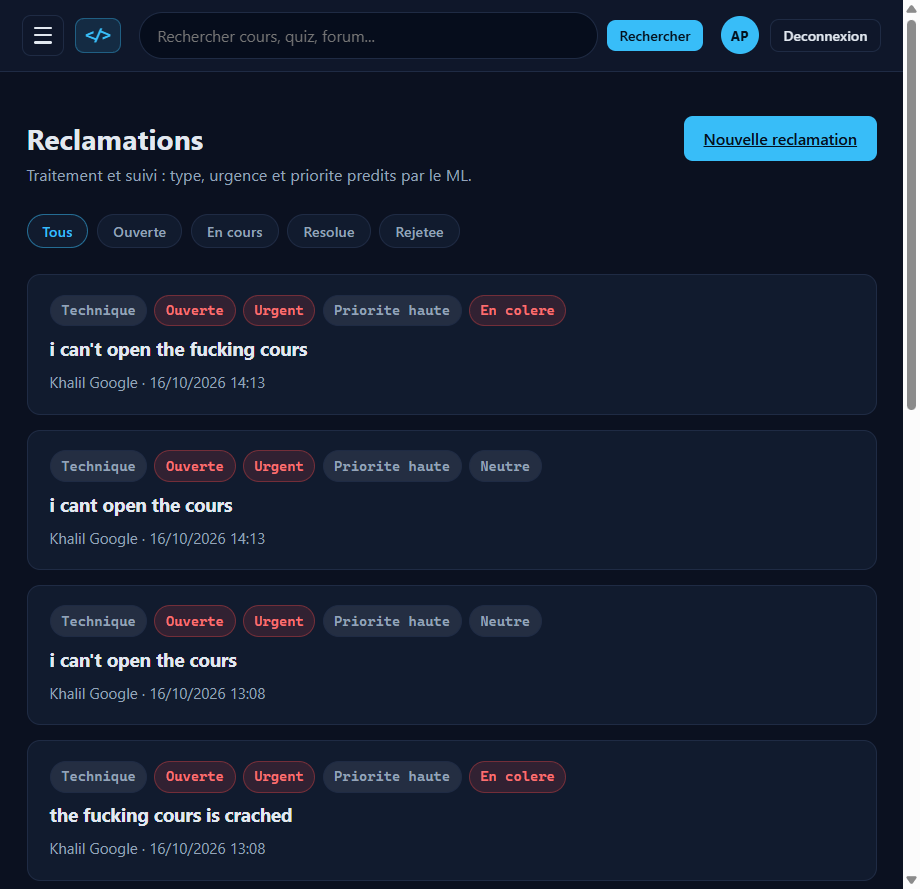
\includegraphics[width=0.92\textwidth]{app/S5-reclamations-liste.png}
  \caption{Capture Promptly --- tags ML type / urgence / priorite / emotion sur la liste}
  \label{fig:s5-ml-liste}
\end{figure}

\begin{promptbox}[title={Correction classification}]
\ldots when i type same urgence in the objet and the description u class it
not urgence \ldots don't make them all urgence make it about the object and
description
\end{promptbox}

\begin{resultbox}[title={Resultat}]
Modele reentraine : classification basee sur le texte objet+description
(ex.\ quiz/deadline $\rightarrow$ technique / urgent ; suggestion calme
$\rightarrow$ non urgent).
\end{resultbox}

\begin{figure}[H]
  \centering
  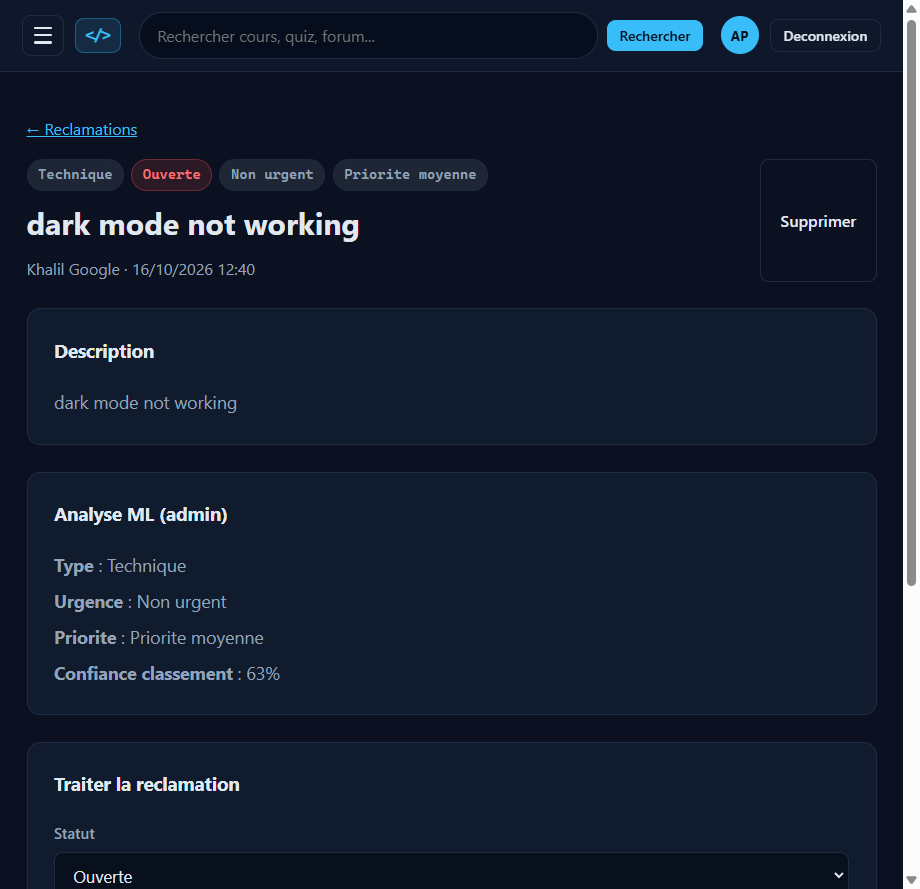
\includegraphics[width=0.92\textwidth]{app/S5-reclamation-ml.png}
  \caption{Capture Promptly --- detail avec classification ML (objet+description)}
  \label{fig:s5-ml-detail}
\end{figure}

\begin{promptbox}
ok now add emotion detaction in the reclation from the way he write the ia
will told the admine is this persone angry or happy ..... use free api
\end{promptbox}

\begin{resultbox}[title={Resultat}]
Emotion (En colere / Content / Triste / \ldots) via Hugging Face Inference
+ fallback lexique local, dans le backend Spring. Admin seulement.
Panneau << Analyse ML (admin) >> : type, urgence, priorite, confiance.
\end{resultbox}

\begin{figure}[H]
  \centering
  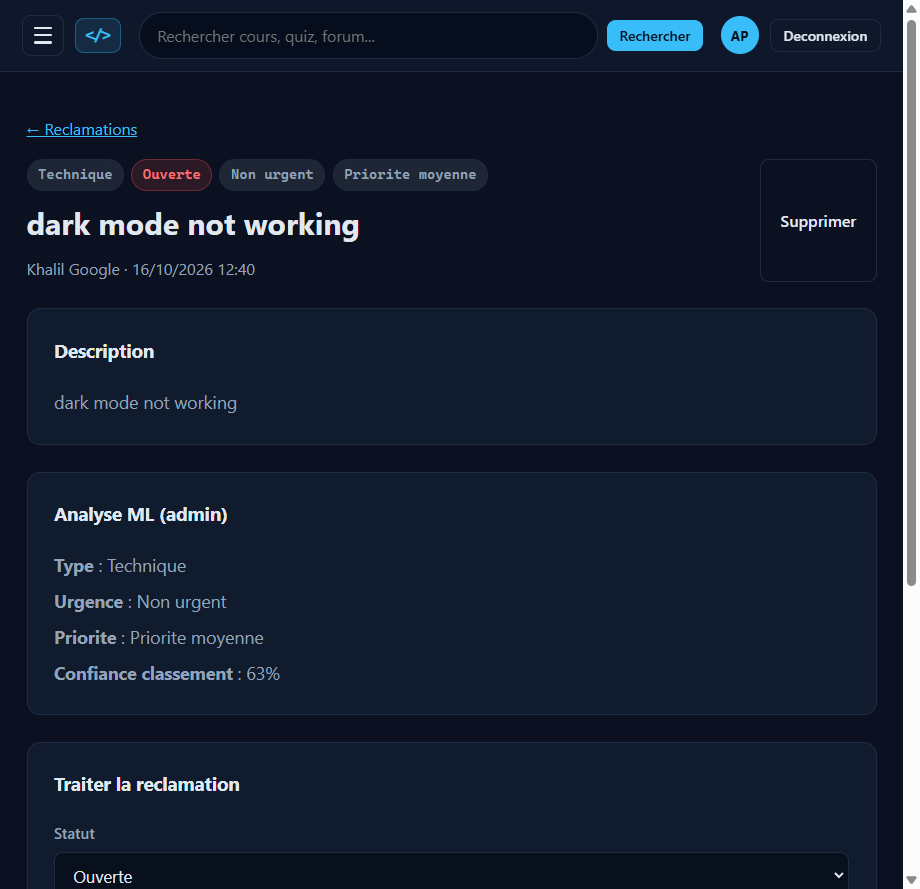
\includegraphics[width=0.92\textwidth]{app/S5-reclamation-ml.png}
  \caption{Capture Promptly --- detail reclamation avec Analyse ML (admin)}
  \label{fig:s5-ml}
\end{figure}

\begin{problembox}[title={Probleme puis correction}]
Emotion reste << Neutre >> malgre un texte agressif. \\
\textbf{Causes :} token HF ecrase / lexique sans mots vulgaires EN. \\
\textbf{Correction :} token local prioritaire + lexique enrichi
$\rightarrow$ detection << En colere >>.
\end{problembox}

%----------------------------------------------------------------------
\subsection{S6 --- Layout (navbar / sidebar)}
\label{sec:s6}

\begin{promptbox}
add side bar and make the nave bar have the login information and the name of
the website and searsh bar
\end{promptbox}

\begin{resultbox}[title={Resultat}]
Sidebar (navigation) + top bar (Promptly, recherche, infos login / logout).
\end{resultbox}

\begin{figure}[H]
  \centering
  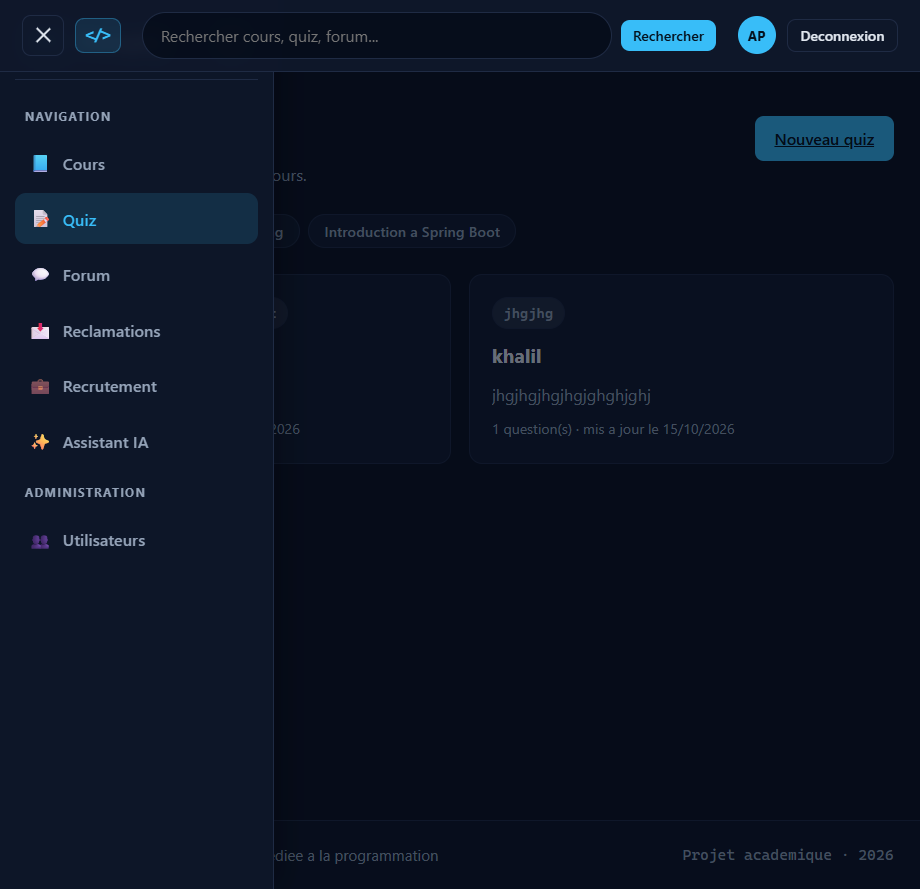
\includegraphics[width=0.92\textwidth]{app/S6-layout-initial.png}
  \caption{Capture Promptly --- layout sidebar + navbar + recherche}
  \label{fig:s6-initial}
\end{figure}

\begin{promptbox}
make the side bar with toggel open and close when i click it
\end{promptbox}

\begin{problembox}
when i click the side bar no thing is happen --- host/overlay bloquait les
clics.
\end{problembox}

\begin{resultbox}[title={Resultat apres correction}]
Bouton menu ouvre/ferme la sidebar ; backdrop mobile ; hard refresh.
\end{resultbox}

\begin{figure}[H]
  \centering
  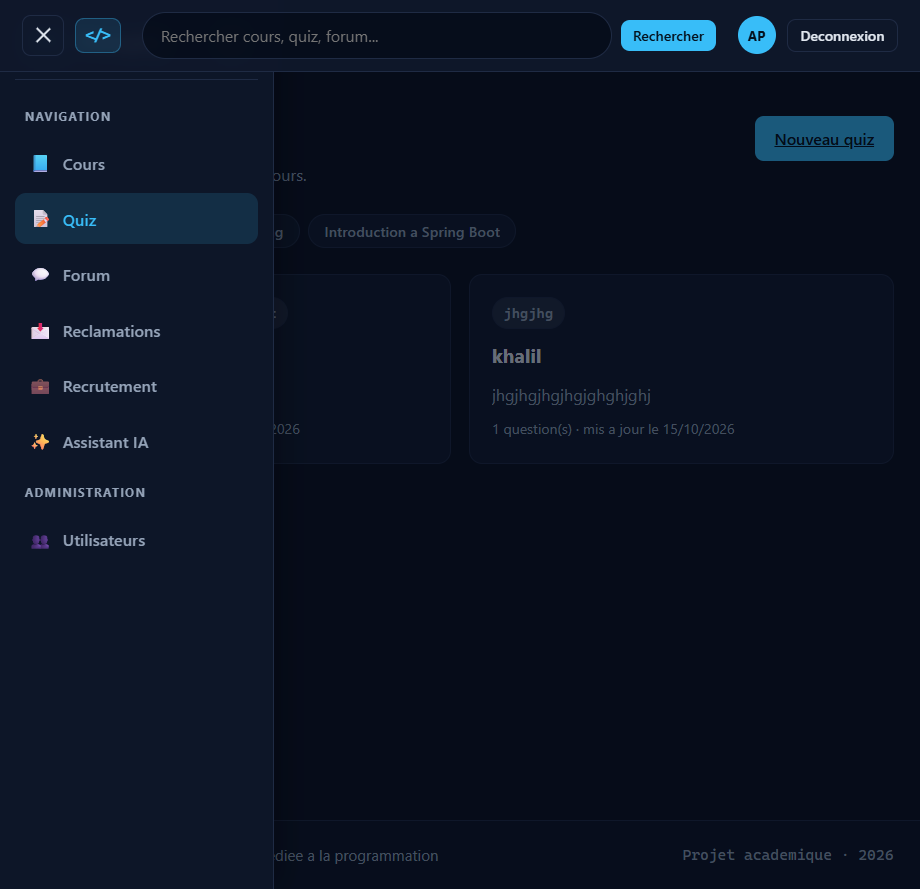
\includegraphics[width=0.92\textwidth]{app/S6-sidebar-navbar.png}
  \caption{Capture Promptly --- sidebar ouverte + navbar (recherche, profil)}
  \label{fig:s6-layout}
\end{figure}

%----------------------------------------------------------------------
\subsection{S7 --- IA pedagogique (Ollama : resume, flashcards)}
\label{sec:s7}

\begin{promptbox}
i download ollama in the pc so make the resumer with ollama
\end{promptbox}

\begin{resultbox}[title={Resultat}]
Bouton << Resumer automatiquement >> sur cours/chapitre PDF :
PDFBox $\rightarrow$ Ollama (\texttt{llama3.2:3b}) $\rightarrow$ resume.
\end{resultbox}

\begin{figure}[H]
  \centering
  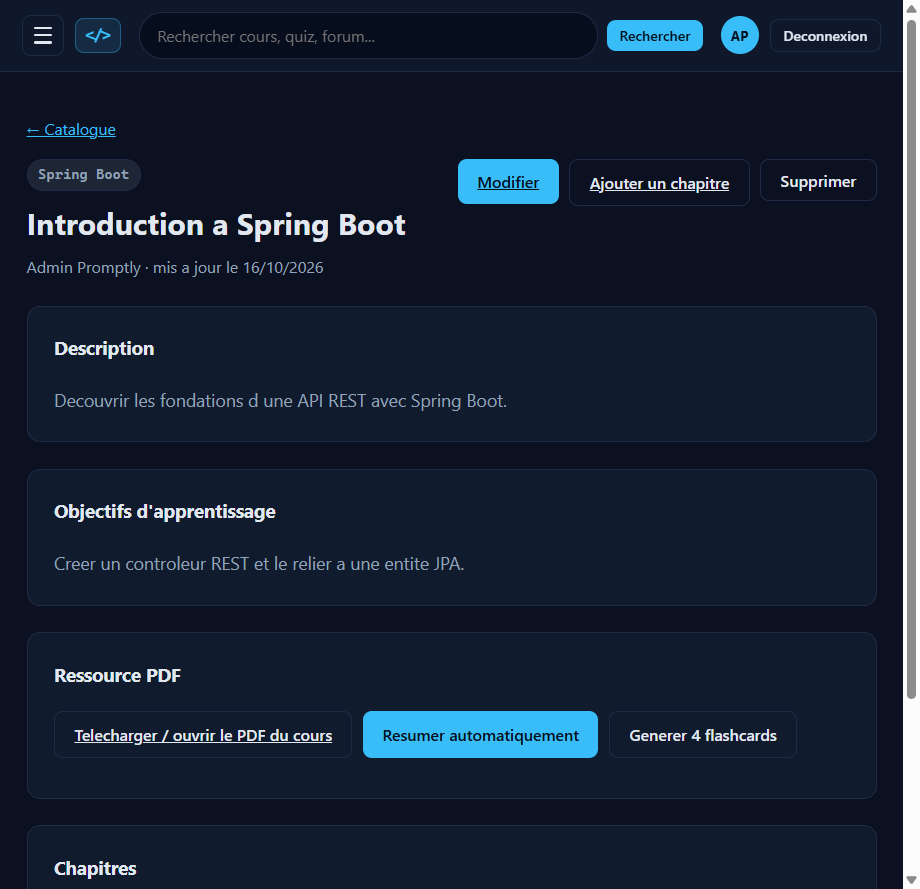
\includegraphics[width=0.92\textwidth]{app/S7-cours-ollama.png}
  \caption{Capture Promptly --- bouton Resumer automatiquement (Ollama)}
  \label{fig:s7-resume}
\end{figure}

\begin{promptbox}
and give like flush card of the cours read the pdf then give me 4 flash card
\ldots when i click them the card turn and i read the tips
\end{promptbox}

\begin{resultbox}[title={Resultat}]
<< Generer 4 flashcards >> : 4 cartes recto/verso (titre / tip) depuis le PDF.
Boutons visibles sur la fiche cours (avec le PDF).
\end{resultbox}

\begin{figure}[H]
  \centering
  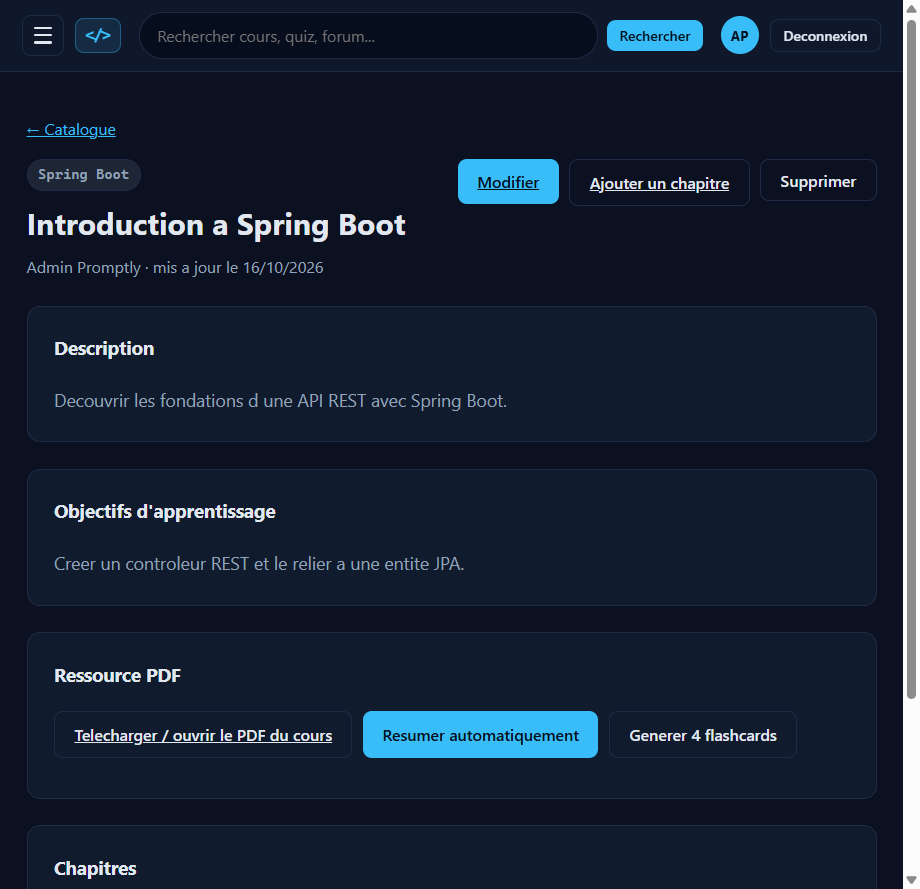
\includegraphics[width=0.92\textwidth]{app/S7-resume-flashcards.png}
  \caption{Capture Promptly --- Generer 4 flashcards (Ollama)}
  \label{fig:s7-flash}
\end{figure}

\begin{problembox}
Impossible d'interpreter les flashcards (400) ; cartes invisibles (CSS 3D).
\textbf{Corrections :} parsing JSON Ollama renforce ; CSS flip simplifie.
\end{problembox}

%----------------------------------------------------------------------
\subsection{S8 --- Assistant IA (chatbot)}
\label{sec:s8}

\begin{promptbox}
assistance ia make chatbot general for the aplication make it like llm
\end{promptbox}

\begin{resultbox}[title={Resultat}]
Page \texttt{/ia} : chat general via \texttt{POST /api/ai/chat} (Ollama),
historique de conversation, suggestions. Necessite Ollama + modele local.
\end{resultbox}

\begin{figure}[H]
  \centering
  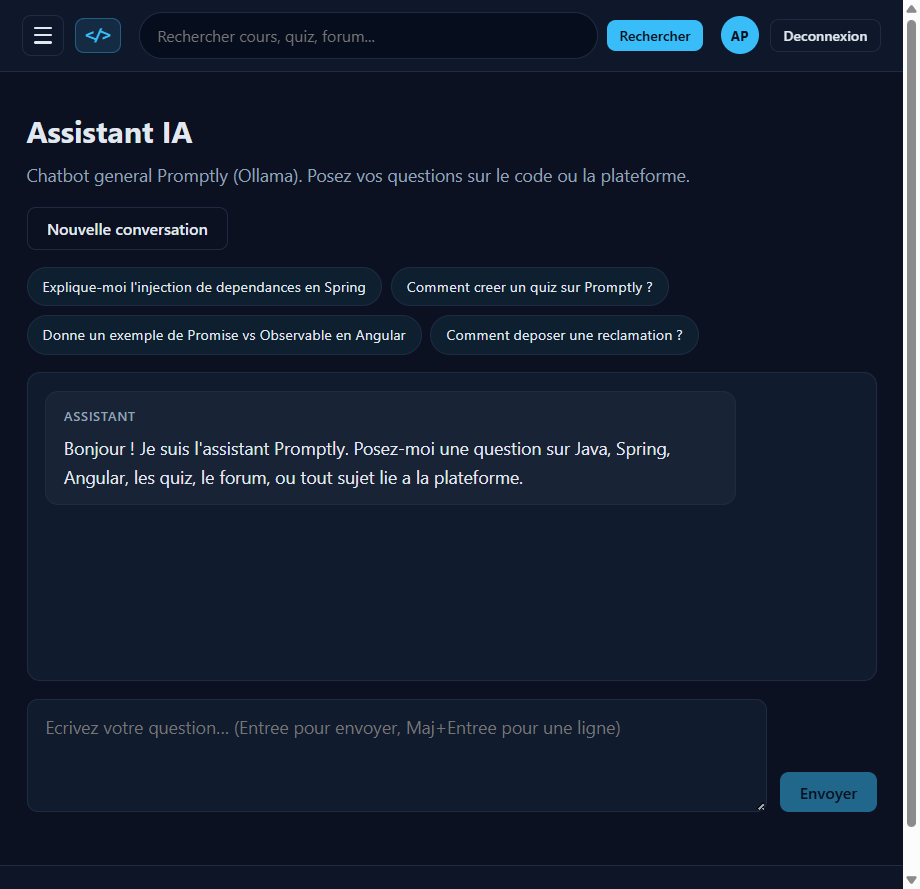
\includegraphics[width=0.92\textwidth]{app/S8-assistant-ia.png}
  \caption{Capture Promptly --- Assistant IA (chatbot Ollama)}
  \label{fig:s8-assistant}
\end{figure}

%----------------------------------------------------------------------
\subsection{S9 --- Recrutement + matching CV}
\label{sec:s9}

\begin{promptbox}
ok we need to add other gestion like recretment the admine make recretment
then make the employee see the offre and add his cv then the admine see how
aplly the offre and see his cv
\end{promptbox}

\begin{resultbox}[title={Resultat}]
Module \texttt{/recrutement} : admin cree offres ; candidats postulent avec
CV PDF ; admin voit candidatures + CV + statuts.
\end{resultbox}

\begin{figure}[H]
  \centering
  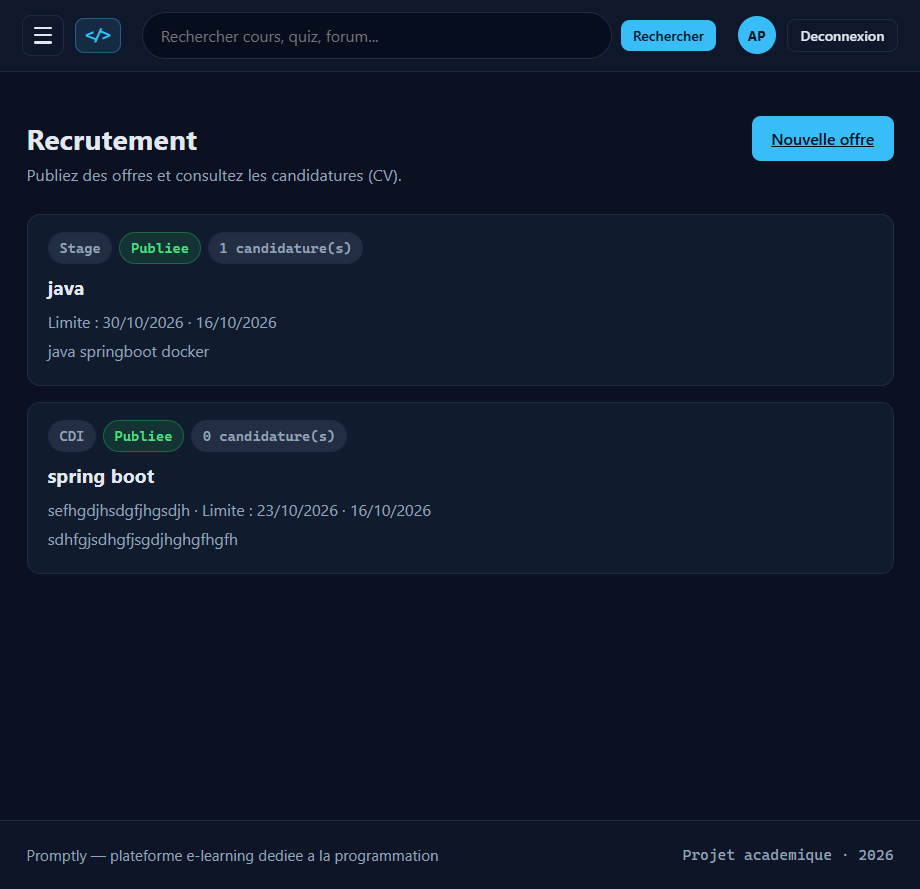
\includegraphics[width=0.92\textwidth]{app/S9-recrutement.png}
  \caption{Capture Promptly --- liste des offres de recrutement}
  \label{fig:s9-recrut}
\end{figure}

\begin{promptbox}
good now add part of skills and experience in the offre form then when the
employee upload his cv make matching cv with the skkils in the offre and the
skills in the cv use api with token to make this and be sure the api free
\end{promptbox}

\begin{resultbox}[title={Resultat (version initiale)}]
Skills + experience sur l'offre ; matching via Hugging Face
(\texttt{bart-large-mnli}) $\rightarrow$ score \%, competences
matched/missing.
\end{resultbox}

\begin{figure}[H]
  \centering
  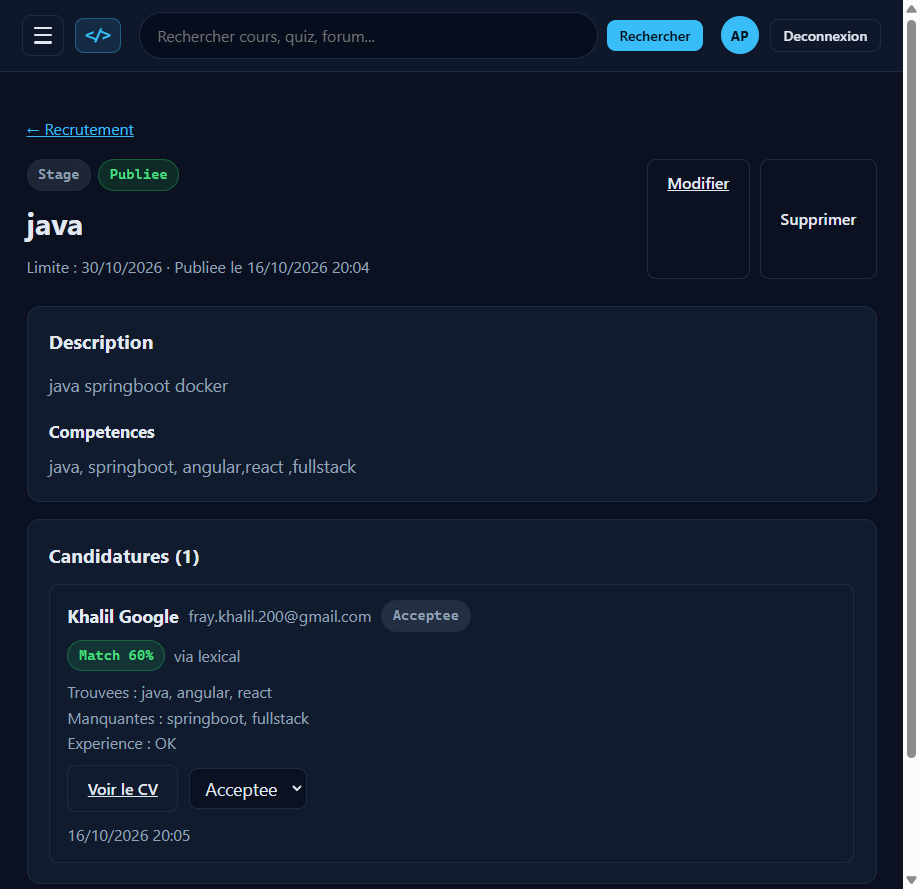
\includegraphics[width=0.92\textwidth]{app/S9-offre-match.png}
  \caption{Capture Promptly --- offre avec competences et score de matching CV}
  \label{fig:s9-match-hf}
\end{figure}

\begin{promptbox}[title={Correction --- changement d'API}]
can u relpalce Hugging Face just in this gestion with other pai to make
matching cv ?
\end{promptbox}

\begin{resultbox}[title={Resultat}]
Matching CV bascule sur \textbf{Google Gemini} (cle gratuite AI Studio).
HF reste pour l'emotion des reclamations. Fallback mots-cles si API down.
Admin voit le score Match \%, competences trouvees / manquantes.
\end{resultbox}

\begin{figure}[H]
  \centering
  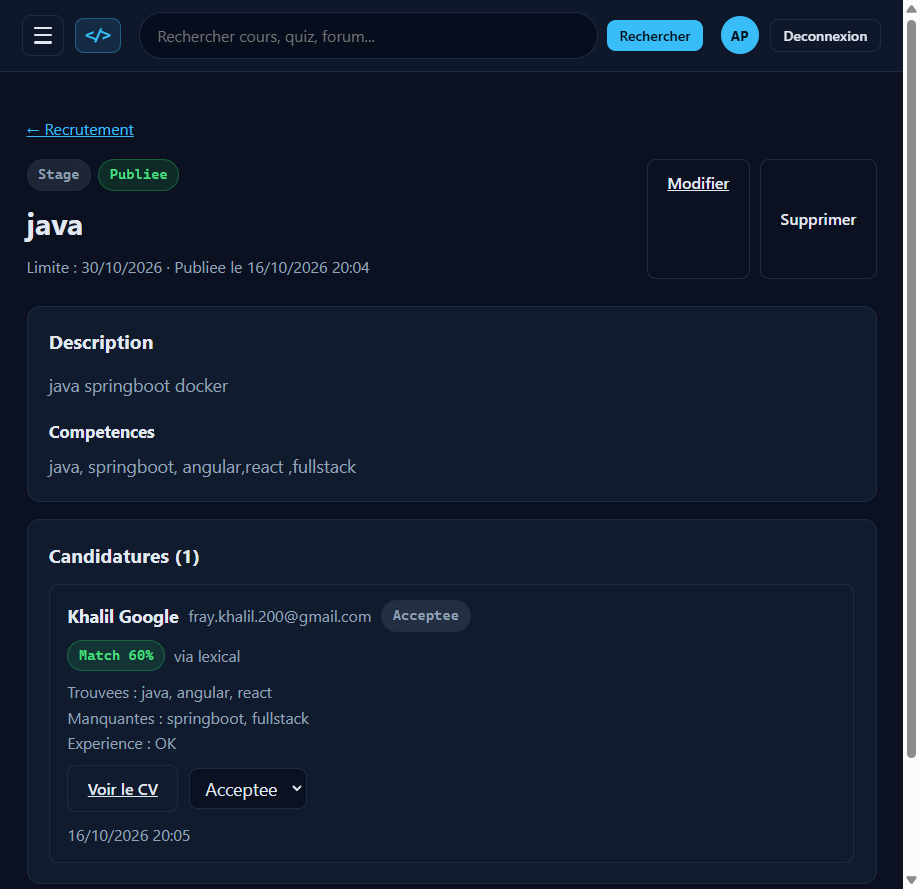
\includegraphics[width=0.92\textwidth]{app/S9-offre-match.png}
  \caption{Capture Promptly --- offre avec matching CV (score + competences)}
  \label{fig:s9-match}
\end{figure}

%----------------------------------------------------------------------
\section{Synthese des sessions}

\begin{table}[H]
\centering
\begin{tabular}{@{}clp{7.5cm}@{}}
\toprule
Session & Gestion & Resultat principal \\
\midrule
S0 & Fondation & Spring Boot + Angular + MySQL + health \\
S1 & Auth (+ Google) & JWT, roles, Sign-In Google \\
S2 & Cours / chapitres & CRUD, image, PDF \\
S3 & Quiz + ML & QCM, Ollama, timers, GUESS/KNOW \\
S4 & Forum & Posts, reactions, Sightengine, TextGears \\
S5 & Reclamations & ML type/urgence + emotion HF \\
S6 & Layout & Sidebar / navbar / recherche \\
S7 & Resume / flashcards & Ollama + PDFBox \\
S8 & Assistant IA & Chatbot Ollama \\
S9 & Recrutement & Offres, CV, matching Gemini \\
\bottomrule
\end{tabular}
\caption{Recapitulatif des gestions documentees depuis l'historique Cursor}
\end{table}

Chaque resultat ci-dessus est illustre par une \textbf{capture de la
plateforme Promptly} (\texttt{figures/app/}). Des captures Cursor
(prompt dans le chat Agent) restent optionnelles dans
\texttt{figures/cursor/}.

\chapter{IA integree a l'application}
\label{ch:app}

Ce chapitre decrit \textbf{comment l'intelligence artificielle est utilisee
dans le produit Promptly} (cote application), et non comment le code a ete
genere avec Cursor / Claude / Grok. Deux familles d'outils coexistent :
\begin{itemize}
  \item \textbf{Ollama} : modele de langage local (LLM) ;
  \item \textbf{APIs externes} et \textbf{microservices ML} : services
        specialises (moderation, emotion, matching, prediction).
\end{itemize}

Les cles API sont stockees dans
\texttt{application-local.properties} (fichier gitignore), jamais dans le
depot Git. Documentation detaillee : \texttt{docs/apis-et-tokens.md}.

\section{Vue d'ensemble des fonctionnalites}

\begin{table}[H]
\centering
\begin{tabular}{@{}p{3.8cm}p{4cm}p{5.2cm}@{}}
\toprule
Fonctionnalite & Technologie & Role \\
\midrule
Resume PDF & Ollama + PDFBox & Resume automatique d'un cours / chapitre \\
Flashcards & Ollama + PDFBox & 4 cartes pedagogiques depuis le PDF \\
Generation de quiz & Ollama & 10 QCM a partir du titre / cours / PDF \\
Assistant IA & Ollama & Chatbot general dans l'application \\
Emotion reclamations & Hugging Face & Ton (colere, neutre, \ldots) pour l'admin \\
Censure forum & Sightengine & Insultes remplacees par \texttt{***} \\
Auto-correct forum & TextGears & Orthographe / grammaire a la publication \\
Matching CV / offre & Google Gemini & Score competences + experience \\
GUESS / KNOW quiz & ml-integrity (:8090) & Reponse au hasard vs connue \\
Type / urgence & ml-complaints (:8091) & Labels admin sur reclamations \\
\bottomrule
\end{tabular}
\caption{Fonctionnalites d'IA integrees a Promptly}
\end{table}

\section{Ollama --- LLM local}

\subsection{Pourquoi Ollama}

Ollama permet d'executer un modele de langage \textbf{sur la machine de
developpement} (\texttt{http://localhost:11434}), sans cout API pour les
fonctions pedagogiques centrales. Les donnees des PDF et des conversations
restent locales. Modele utilise : \texttt{llama3.2:3b} (ou equivalent
installe via \texttt{ollama pull}).

Extraction de texte des PDF : bibliotheque Java \textbf{Apache PDFBox}
dans le backend Spring Boot, avant envoi du texte a Ollama.

\subsection{Resume automatique de PDF}

Sur la fiche d'un \textbf{cours} ou d'un \textbf{chapitre} ayant un PDF :
\begin{enumerate}
  \item l'utilisateur clique sur << Resumer automatiquement >> ;
  \item le backend extrait le texte du PDF (tronque si trop long) ;
  \item Ollama produit un resume en francais ;
  \item le resume s'affiche sous la section PDF.
\end{enumerate}
Endpoints typiques :
\texttt{POST /api/ai/courses/\{id\}/summarize-pdf} et equivalent chapitre.
Limitation : un PDF scanne (image seule, sans texte selectable) ne peut pas
etre resume.

\subsection{Flashcards}

Meme flux PDF $\rightarrow$ texte $\rightarrow$ Ollama, avec une consigne
demandant \textbf{4 flashcards} (recto = titre / question, verso = tip).
Bouton << Generer 4 flashcards >> ; l'utilisateur retourne les cartes dans
l'interface Angular. Le backend parse la reponse JSON d'Ollama (avec
fallbacks si le format est imparfait).

\subsection{Generation de quiz (10 questions)}

Dans le formulaire << Nouveau quiz >>, apres titre, description et choix
du cours (chapitre optionnel) :
\begin{enumerate}
  \item clic sur << Generer 10 questions avec IA >> ;
  \item Ollama recoit titre, description et contenu du cours / chapitre / PDF ;
  \item 10 QCM sont proposes ; l'enseignant peut les modifier avant creation.
\end{enumerate}
La generation peut prendre 30 a 90 secondes selon la machine.

\subsection{Assistant IA (chatbot)}

Page \texttt{/ia} : chatbot general de la plateforme.
\begin{itemize}
  \item Backend : \texttt{POST /api/ai/chat} avec historique de conversation ;
  \item Frontend : bulles de chat, suggestions de questions, envoi par Entree ;
  \item Pre-requis : Ollama demarre et modele telecharge.
\end{itemize}
L'assistant repond a des questions sur Java, Spring, Angular, le fonctionnement
de Promptly, etc. Ce n'est pas un remplacement du professeur : c'est une aide
contextuelle integree a l'application.

\section{APIs externes}

\subsection{Hugging Face --- emotion des reclamations}

\textbf{Usage.} Analyser le \textbf{ton} d'une reclamation (En colere, Content,
Triste, Inquiet, Surpris, Neutre) a partir du texte objet + description.

\textbf{Qui voit le resultat.} Uniquement l'\textbf{administrateur} (panneau
Analyse ML). L'etudiant qui depose la reclamation ne voit pas l'emotion.

\textbf{Technique.} Appel Inference API Hugging Face depuis le backend Spring
(\texttt{ComplaintEmotionService}). Token :
\texttt{promptly.emotion.hf-token}. Si l'API est indisponible, un
\textbf{lexique local} FR/EN sert de secours.

\subsection{Sightengine --- moderation du forum}

\textbf{Usage.} Detecter les insultes / gros mots dans les \textbf{posts} et
\textbf{commentaires} du forum, puis les remplacir par \texttt{***} (plutot
que de rejeter le message).

\textbf{Technique.} API Sightengine (plan gratuit) avec \texttt{api-user} et
\texttt{api-secret} dans \texttt{application-local.properties}. Service Java :
\texttt{ProfanityFilterService}. Sans cles : liste locale de mots.

\subsection{TextGears --- auto-correction du forum}

\textbf{Usage.} Corriger l'orthographe et la grammaire \textbf{a la
publication} d'un post ou d'un commentaire (avant la censure Sightengine).

\textbf{Technique.} API TextGears avec cle
\texttt{promptly.spellcheck.api-key} ; langue configurable
(\texttt{fr-FR} ou \texttt{en-US}). Service : \texttt{SpellCorrectService}.
Le professeur exigeait une API avec token : TextGears a ete retenu apres
essais d'autres fournisseurs (LanguageTool Premium, GrammarBot ferme, etc.).

\subsection{Google Gemini --- matching CV / offre}

\textbf{Usage.} Dans le module \textbf{Recrutement}, apres depot d'un CV PDF
sur une offre contenant des \textbf{competences} (et eventuellement une
experience) :
\begin{enumerate}
  \item extraction du texte du CV (PDFBox) ;
  \item Gemini compare le CV aux competences de l'offre ;
  \item le backend stocke un \textbf{score Match \%}, les competences
        trouvees / manquantes, et un indicateur d'experience.
\end{enumerate}
Visible par l'\textbf{admin} sur la fiche de candidature. Cle gratuite AI Studio :
\texttt{promptly.cv-match.api-key}. Sans cle : matching lexical (mots-cles)
en secours. Hugging Face n'est \textbf{plus} utilise pour cette fonction
(uniquement pour l'emotion).

\section{Microservices ML locaux (Python)}

\subsection{ml-integrity (port 8090) --- GUESS / KNOW}

Lorsqu'un etudiant passe un quiz (une question a la fois, avec minuteurs),
le service Python \texttt{ml-integrity} (scikit-learn, RandomForest) predit
si la reponse est :
\begin{itemize}
  \item \texttt{GUESS} : reponse au hasard ;
  \item \texttt{KNOW} : reponse probablement connue.
\end{itemize}
Features utilisees : temps passe, changements de reponse, etc.
\textbf{Seul l'enseignant} voit ces labels (Detail + analyse ML). Une
reponse fausse est forcee en \texttt{GUESS}. Si le service est arrete, Spring
applique une heuristique locale.

\subsection{ml-complaints (port 8091) --- type, urgence, priorite}

A chaque nouvelle reclamation, le service \texttt{ml-complaints} predit :
\begin{itemize}
  \item \textbf{type} (technique, pedagogique, compte, \ldots) ;
  \item \textbf{urgence} (urgent / non urgent) ;
  \item \textbf{priorite} (haute / moyenne / \ldots).
\end{itemize}
L'etudiant ne remplit que l'objet et la description ; les labels sont
reserves a l'admin. La classification s'appuie sur le \textbf{texte} (pas
uniquement sur des mots-cles fixes). Emotion = service HF separe (voir
ci-dessus), pas ce microservice.

\section{Synthese}

\begin{itemize}
  \item \textbf{Ollama} couvre le coeur pedagogique : resume, flashcards,
        generation de quiz, assistant chatbot --- gratuit et local.
  \item \textbf{APIs externes} couvrent des besoins specialises : emotion
        (HF), moderation (Sightengine), orthographe (TextGears), matching CV
        (Gemini).
  \item \textbf{ML Python} couvre des predictions metier : integrite des
        reponses au quiz, tri des reclamations.
  \item En cas d'indisponibilite d'une API ou d'un service ML, des
        \textbf{fallbacks} locaux limitent la panne de l'application.
\end{itemize}

\chapter{Conclusion}
\label{ch:conclusion}

\section{Bilan}

L'IA a ete utilisee sur \textbf{deux faces} :
\begin{itemize}
  \item \textbf{Developpement} : ChatGPT pour amorcer le cahier des prompts ;
        editeur \textbf{Cursor} avec modeles \textbf{Claude} et \textbf{Grok}
        pour implementer et corriger le code de facon iterative ;
  \item \textbf{Produit} : Ollama et APIs (HF, Sightengine, TextGears, Gemini)
        plus des modeles ML locaux pour des besoins metier precis.
\end{itemize}

\section{Limites}

\begin{itemize}
  \item les modeles peuvent proposer du code incorrect : verification et prompts
        de correction sont indispensables ;
  \item les APIs gratuites ont des quotas et peuvent etre indisponibles ;
  \item les captures et prompts doivent etre reels (pas reconstitues).
\end{itemize}

\section{Perspectives}

Enrichir le journal de prompts avec toutes les sessions (en indiquant Claude ou
Grok), completer les figures, et ajouter d'autres captures des fonctionnalites
IA en situation reelle d'utilisation.


\end{document}
